\documentclass[a4paper,11pt,oneside]{memoir}

% Castellano
\usepackage[spanish]{babel}
\selectlanguage{spanish}
\usepackage[utf8]{inputenc}
\usepackage{placeins}

\usepackage{listings}

\RequirePackage{booktabs}
\RequirePackage[table]{xcolor}
\RequirePackage{xtab}
\RequirePackage{multirow}

% Links
\usepackage[colorlinks]{hyperref}
\hypersetup{
	allcolors = {red}
}

% Ecuaciones
\usepackage{amsmath}

% Rutas de fichero / paquete
\newcommand{\ruta}[1]{{\sffamily #1}}

% Párrafos
\nonzeroparskip


% Imagenes
\usepackage{graphicx}
\newcommand{\imagen}[2]{
	\begin{figure}[!h]
		\centering
		\includegraphics[width=0.9\textwidth]{#1}
		\caption{#2}\label{fig:#1}
	\end{figure}
	\FloatBarrier
}

\newcommand{\imagenflotante}[2]{
	\begin{figure}%[!h]
		\centering
		\includegraphics[width=0.9\textwidth]{#1}
		\caption{#2}\label{fig:#1}
	\end{figure}
}



% El comando \figura nos permite insertar figuras comodamente, y utilizando
% siempre el mismo formato. Los parametros son:
% 1 -> Porcentaje del ancho de página que ocupará la figura (de 0 a 1)
% 2 --> Fichero de la imagen
% 3 --> Texto a pie de imagen
% 4 --> Etiqueta (label) para referencias
% 5 --> Opciones que queramos pasarle al \includegraphics
% 6 --> Opciones de posicionamiento a pasarle a \begin{figure}
\newcommand{\figuraConPosicion}[6]{%
  \setlength{\anchoFloat}{#1\textwidth}%
  \addtolength{\anchoFloat}{-4\fboxsep}%
  \setlength{\anchoFigura}{\anchoFloat}%
  \begin{figure}[#6]
    \begin{center}%
      \Ovalbox{%
        \begin{minipage}{\anchoFloat}%
          \begin{center}%
            \includegraphics[width=\anchoFigura,#5]{#2}%
            \caption{#3}%
            \label{#4}%
          \end{center}%
        \end{minipage}
      }%
    \end{center}%
  \end{figure}%
}

%
% Comando para incluir imágenes en formato apaisado (sin marco).
\newcommand{\figuraApaisadaSinMarco}[5]{%
  \begin{figure}%
    \begin{center}%
    \includegraphics[angle=90,height=#1\textheight,#5]{#2}%
    \caption{#3}%
    \label{#4}%
    \end{center}%
  \end{figure}%
}
% Para las tablas
\newcommand{\otoprule}{\midrule [\heavyrulewidth]}
%
% Nuevo comando para tablas pequeñas (menos de una página).
\newcommand{\tablaSmall}[5]{%
 \begin{table}
  \begin{center}
   \rowcolors {2}{gray!35}{}
   \begin{tabular}{#2}
    \toprule
    #4
    \otoprule
    #5
    \bottomrule
   \end{tabular}
   \caption{#1}
   \label{tabla:#3}
  \end{center}
 \end{table}
}

%
% Nuevo comando para tablas pequeñas (menos de una página).
\newcommand{\tablaSmallSinColores}[5]{%
 \begin{table}[H]
  \begin{center}
   \begin{tabular}{#2}
    \toprule
    #4
    \otoprule
    #5
    \bottomrule
   \end{tabular}
   \caption{#1}
   \label{tabla:#3}
  \end{center}
 \end{table}
}

\newcommand{\tablaApaisadaSmall}[5]{%
\begin{landscape}
  \begin{table}
   \begin{center}
    \rowcolors {2}{gray!35}{}
    \begin{tabular}{#2}
     \toprule
     #4
     \otoprule
     #5
     \bottomrule
    \end{tabular}
    \caption{#1}
    \label{tabla:#3}
   \end{center}
  \end{table}
\end{landscape}
}

%
% Nuevo comando para tablas grandes con cabecera y filas alternas coloreadas en gris.
\newcommand{\tabla}[6]{%
  \begin{center}
    \tablefirsthead{
      \toprule
      #5
      \otoprule
    }
    \tablehead{
      \multicolumn{#3}{l}{\small\sl continúa desde la página anterior}\\
      \toprule
      #5
      \otoprule
    }
    \tabletail{
      \hline
      \multicolumn{#3}{r}{\small\sl continúa en la página siguiente}\\
    }
    \tablelasttail{
      \hline
    }
    \bottomcaption{#1}
    \rowcolors {2}{gray!35}{}
    \begin{xtabular}{#2}
      #6
      \bottomrule
    \end{xtabular}
    \label{tabla:#4}
  \end{center}
}

%
% Nuevo comando para tablas grandes con cabecera.
\newcommand{\tablaSinColores}[6]{%
  \begin{center}
    \tablefirsthead{
      \toprule
      #5
      \otoprule
    }
    \tablehead{
      \multicolumn{#3}{l}{\small\sl continúa desde la página anterior}\\
      \toprule
      #5
      \otoprule
    }
    \tabletail{
      \hline
      \multicolumn{#3}{r}{\small\sl continúa en la página siguiente}\\
    }
    \tablelasttail{
      \hline
    }
    \bottomcaption{#1}
    \begin{xtabular}{#2}
      #6
      \bottomrule
    \end{xtabular}
    \label{tabla:#4}
  \end{center}
}

%
% Nuevo comando para tablas grandes sin cabecera.
\newcommand{\tablaSinCabecera}[5]{%
  \begin{center}
    \tablefirsthead{
      \toprule
    }
    \tablehead{
      \multicolumn{#3}{l}{\small\sl continúa desde la página anterior}\\
      \hline
    }
    \tabletail{
      \hline
      \multicolumn{#3}{r}{\small\sl continúa en la página siguiente}\\
    }
    \tablelasttail{
      \hline
    }
    \bottomcaption{#1}
  \begin{xtabular}{#2}
    #5
   \bottomrule
  \end{xtabular}
  \label{tabla:#4}
  \end{center}
}



\definecolor{cgoLight}{HTML}{EEEEEE}
\definecolor{cgoExtralight}{HTML}{FFFFFF}

%
% Nuevo comando para tablas grandes sin cabecera.
\newcommand{\tablaSinCabeceraConBandas}[5]{%
  \begin{center}
    \tablefirsthead{
      \toprule
    }
    \tablehead{
      \multicolumn{#3}{l}{\small\sl continúa desde la página anterior}\\
      \hline
    }
    \tabletail{
      \hline
      \multicolumn{#3}{r}{\small\sl continúa en la página siguiente}\\
    }
    \tablelasttail{
      \hline
    }
    \bottomcaption{#1}
    \rowcolors[]{1}{cgoExtralight}{cgoLight}

  \begin{xtabular}{#2}
    #5
   \bottomrule
  \end{xtabular}
  \label{tabla:#4}
  \end{center}
}




\graphicspath{ {./img/} }

% Capítulos
\chapterstyle{bianchi}
\newcommand{\capitulo}[2]{
	\setcounter{chapter}{#1}
	\setcounter{section}{0}
	\chapter*{#2}
	\addcontentsline{toc}{chapter}{#2}
	\markboth{#2}{#2}
}

% Apéndices
\renewcommand{\appendixname}{Apéndice}
\renewcommand*\cftappendixname{\appendixname}

\newcommand{\apendice}[1]{
	%\renewcommand{\thechapter}{A}
	\chapter{#1}
}

\renewcommand*\cftappendixname{\appendixname\ }

% Formato de portada
\makeatletter
\usepackage{xcolor}
\newcommand{\tutor}[1]{\def\@tutor{#1}}
\newcommand{\course}[1]{\def\@course{#1}}
\definecolor{cpardoBox}{HTML}{E6E6FF}
\def\maketitle{
  \null
  \thispagestyle{empty}
  % Cabecera ----------------
\noindent
\includegraphics[width=\textwidth]{cabecera}\vspace{1cm}%
  \vfill
  % Título proyecto y escudo informática ----------------
  \colorbox{cpardoBox}{%
    \begin{minipage}{.8\textwidth}
      \vspace{.5cm}\Large
      \begin{center}
      \textbf{TFM del Máster en Ingeniería Informática}\vspace{.6cm}\\
      \textbf{\LARGE\@title{}}
      \end{center}
      \vspace{.2cm}
    \end{minipage}

  }%
  \hfill\begin{minipage}{.20\textwidth}
    
\includegraphics[width=\textwidth]{escudoInfor}
  \end{minipage}
  \vfill
  % Datos de alumno, curso y tutores ------------------
  \begin{center}%
  {%
    \noindent\LARGE
    Presentado por \@author{}\\ 
    en Universidad de Burgos --- \@date{}\\
    Tutores: \@tutor{} y \coTutorTFM \\
  }%
  \end{center}%
  \null
  \cleardoublepage
  }
\makeatother

\newcommand{\nombre}{David Moreno del Hoyo} %%% cambio de comando
\newcommand{\fechaEntrega}{10 de febrero de 2017}
\newcommand{\titulo}{Sistema para el registro y análisis de trayectorias semánticas}
\newcommand{\tutorTFM}{Bruno Baruque}
\newcommand{\coTutorTFM}{Santiago Porras}


% Datos de portada
\title{\titulo \\ Documentación Técnica}
\author{\nombre}
\tutor{\tutorTFM}
\date{\fechaEntrega}

\begin{document}

\maketitle



\cleardoublepage



%%%%%%%%%%%%%%%%%%%%%%%%%%%%%%%%%%%%%%%%%%%%%%%%%%%%%%%%%%%%%%%%%%%%%%%%%%%%%%%%%%%%%%%%



\frontmatter


\clearpage

% Indices
\tableofcontents

\clearpage

\listoffigures

\clearpage

%\listoftables

%\clearpage

\mainmatter

\appendix

\apendice{Plan de Proyecto Software}

\section{Introducción}

La planificación de un proyecto software debe incluir los siguientes apartados:

\begin{itemize}
	\item Planificación temporal: tratará de determinar los marcos temporales durante los que el desarrollo tendrá lugar. Es decir, se acordará una fecha de comienzo, y dependiendo de las características a implementar, se propondrá una fecha de finalización. 
	\item Estudio de viabilidad: este estudio trata de calcular los costes que supondrá el desarrollo de la aplicación así como de los inconvenientes legales que puedan plantearse para su posterior puesta en venta.
\end{itemize}

De esta forma se contará con la información que permita controlar los costes y riesgos tomados al comenzar el desarrollo de una aplicación determinada.

\section{Planificación temporal}

El desarrollo del proyecto ha sido basado en la metodología Scrum, por tanto, se trata de un desarrollo ágil. Aunque Scrum define una serie de buenas prácticas a aplicar durante todo el desarrollo, en el proyecto actual no se han aplicado todas y cada una de las mismas. Las aplicadas en este trabajo son:

\begin{itemize}
	\item Desarrollo incremental e iterativo.
	\item Reuniones término de cada \textit{sprint}.
\end{itemize}

El presente trabajo ha sido desarrollado desde el mes de marzo de 2017 hasta el mes de septiembre del mismo año. Los primeros sprints (primero, segundo y tercero) contaron con una duración aproximada de un mes mientras que los finales (cuarto a noveno) se han realizado de forma quincenal. 
Los \textit{sprints} llevados a cabo se muestran a continuación.

\subsection{Sprint 1}
Estudio inicial del estado del arte y documentación sobre la que el proyecto se basa.

\subsection{Sprint 2}
Estudio de los requisitos del sistema, analizando las necesidades de almacenamiento y recuperación de datos. Selección de PostgreSQL y PostGIS como SGBD y extensión del mismo.

\subsection{Sprint 3}
Desarrollo inicial del algoritmo de análisis de rutas, implementando la lectura de ficheros y almacenado en crudo de los datos sobre el sistema.

\subsection{Sprint 4}
Segunda iteración sobre el algoritmo de análisis de rutas para poder separar dichas rutas y descubrir paradas sobre las mismas.

\subsection{Sprint 5}
Tercera iteración sobre el algoritmo, posibilitando la búsqueda de PDIs sobre las paradas detectadas.

\subsection{Sprint 6}
Primer diseño de la interfaz web, diseño de las páginas de carga de ficheros, selección de opciones del algoritmo y resultados finales.

\subsection{Sprint 7}
Implementación de la interfaz según los prototipados iniciales y aplicación de estilos finales.

\subsection{Sprint 8}
Versión inicial de la documentación del proyecto. Adición de página de visualizado de resultados.

\subsection{Sprint 9}
Versión final de la documentación del trabajo, anexos y memoria completados.

\section{Estudio de viabilidad}
El estudio de viabilidad de un proyecto debe estimar la posibilidad de obtener una rentabilidad a partir de los costes y beneficios que produzca el desarrollo de la aplicación.

No obstante, si se desea realizar una aplicación privativa se deben estudiar los términos de las licencias del software de terceros usado en el proyecto.

En los siguientes apartados se realiza tanto un estudio económico como uno legal.

\subsection{Viabilidad económica}
El apartado correspondiente a la viabilidad económica tratará de calcular la rentabilidad económica del proyecto, detallando los costes y estimando la posibilidad de obtención de ingresos. Se estima que la duración del proyecto será de cinco meses.

Dentro del ámbito de los costes incluimos los siguientes apartados:
\begin{itemize}
	\item \textbf{Coste laboral.}
	\item \textbf{Coste de capital:}
	\begin{itemize}
		\item \textbf{Coste de hardware.}
		\item \textbf{Coste de software.}
		\item \textbf{Suministros.}
		\item \textbf{Alquileres.}
		\item \textbf{Material de oficina.}
	\end{itemize}
\end{itemize}		
		
\subsubsection{Coste laboral}

Para el desarrollo del proyecto se contratará a un único programador por un tiempo de cinco meses a jornada completa.

El salario bruto prorrateando las pagas extra será de 1.400 euros mensuales. La empresa deberá de tener en cuenta el pago que le corresponde realizar a la Seguridad Social \cite{bases:info} \cite{tarifas:info} y será el 32,1\% que se aplica sobre la base de cotización, que en este caso será de 1.400 euros. Se desglosa de la siguiente manera:

\begin{itemize}
	\item \textbf{Contingencias comunes:} 23,6%.
	\item \textbf{Desempleo:} 6,7\%. (Contrato de duración determinada.)
	\item \textbf{FOGASA:} 0,2%.
	\item \textbf{Formación Profesional}: 0,6\%.
	\item \textbf{Cotización de AT (Accidentes de Trabajo) y EP (Enfermedad Profesional):} se utiliza la tarifa “a” (personal de trabajos de oficina) corresponde un 0,65\% para IT (Incapacidad Temporal) y un 0,35\% para IMS (Invalidez, Muerte y Supervivencia).

\end{itemize}

El coste laboral por persona y mes será el siguiente:

\begin{itemize}
	\item 1.400 + (1.400*32,1\%)= \textbf{1.849 euros.}
\end{itemize}

Siendo el coste total el calculado a continuación:

\begin{itemize}
	\item 1.849,4*5=\textbf{9.247 euros.}
\end{itemize}

En el momento de la contratación se verá si el programador elegido se puede acoger a algún tipo de bonificación \cite{bonif:info} en las cuotas que paga la empresa a la Seguridad Social, para ello nos informaremos en la siguiente página.


\subsubsection{Coste de capital}
Se adquirirá un equipo a un coste unitario de 1.500 euros siendo la adquisición del equipo una inversión. Este ordenador se podrá utilizar a lo largo de su vida útil para otros proyectos. Las características principales de este ordenador son las siguientes:

\begin{itemize}
	\item \textbf{CPU:} Core i7 de séptima generación.
	\item \textbf{RAM:} 16 GiB de memoria RAM de tipo DDR4.
	\item \textbf{SSD:} 250 GiB de disco en estado sólido.
	\item \textbf{PSU:} Fuente de alimentación de 500W.
	\item \textbf{Monitor:} pantalla plana de 24".
\end{itemize}

Se considera una vida útil de 5 años, siguiendo un método de amortización lineal y un valor residual nulo se podrán contabilizar unos gastos anuales de amortización de 300 euros, que prorrateando por meses corresponderán a 25 euros/mes.

Respecto al coste del \textbf{software}, durante todo el desarrollo de la aplicación, se hará uso de herramientas de software libre que permitan prescindir del pago de licencias privativas. Algunas de las aplicaciones que serán usadas son:

\begin{itemize}
	\item \textbf{Ubuntu 16.04 LTS} como Sistema Operativo.
	\item \textbf{Glassfish} como servidor web.
	\item \textbf{OpenStreetMaps} como fuente de datos y mapas.
	\item \textbf{NetBeans} como IDE de desarrollo.
	\item \textbf{TexMaker} como editor de texto para la documentación.
\end{itemize}

El coste de los \textbf{suministros}, una vez calculados los costes de agua, luz, fibra, etc, ascienden a 125 euros mensuales.

Respecto al coste del \textbf{alquiler}, se estima un coste mensual de 100 euros por el arriendo de una oficina.

Por último, el coste total del \textbf{material de oficina} se calcula en 50 euros.

La suma de todos los costes relacionados con el capital asciende a:

\begin{itemize}
	\item (125 + 100 + 25)*5 + 50 = \textbf{1.300 euros}.
\end{itemize}

El coste total del proyecto ascenderá a la siguiente cantidad:

\begin{itemize}
	\item 9.247 + 1.300 = \textbf{10.547 euros}.
\end{itemize}

La tabla \ref{table:costes} presenta esta información de manera ordenada y clara.

\begin{table}
	\centering
		\begin{tabular}{l*{6}{c}r}
		\hline
			Costes                & Mes & Nº de meses & total \\
		\hline
			Coste laboral 	  	  &		  &  &   \\
			Salario bruto         & 1.400 & 5  & 7.000  \\
			Seguridad Social      & 449.4 & 5 & 2.247\\
		\hline
			Total (coste laboral)	& 1.849,4 & 5 & 9.247   \\
		\hline
			Amortización de Hardware	& 25 & 5 & 125  \\
			Software     & 0 & 0 & 0  \\
			Suministros     & 125 & 5 & 625  \\
			Alquileres     & 100 & 5 & 500  \\
			Material de oficina   & 50  &  & 50 \\
		\hline
			Total (coste de capital)     &  &  &  1.300 \\
		\hline
			Total     &  &  &  10.547  \\
		\hline
	\end{tabular}
	\caption{Costes de desarrollo.}
	\label{table:costes}
\end{table}

\subsubsection{Ingresos estimados}
Para que los costes de desarrollo (contratación de un programador, costes relacionados con las instalaciones y equipos informáticos, etc) sean viables se propone la venta del software desarrollado mediante un sistema de licencias.

Cada licencia podrá ser vendida a un usuario individual o a una empresa. Los costes de licencias serán diferentes puesto que la empresa dispondrá de rappels por volumen de compra.

Se estima que una licencia única podrá tener un coste estimado para un usuario final de 59 euros por licencia anual. Una empresa podrá disponer de un descuento máximo de un 25\%, rebajando el coste de la licencia a 44.25 euros.

Utilizando la fórmula del punto muerto (que nos indica las licencias a vender para que el beneficio sea cero, es decir, a partir de ahí se comienzan a obtener beneficios) y considerando como costes fijos los 10.547 euros y atribuyendo un coste variable por licencia de 3 euros y utilizando el precio menos favorable para la empresa se necesitarán vender 250 licencias para comenzar a obtener beneficio.

La fórmula de PM es la siguiente:

\begin{equation*}
 	PM = \frac{CF}{P - CVu}
\end{equation*}

Siendo los elementos de la fórmula los siguientes:

\begin{itemize}
	\item PM: Punto Muerto.
	\item CF: Coste Fijo.
	\item P: Precio de venta.
	\item CVu: Coste Variable unitario.
\end{itemize}

Según los datos mostrados anteriormente, el número mínimo de licencias a vender para llegar al Punto Muerto será el siguiente:

\begin{equation*}
 	PM = \frac{10.547}{44.25 - 2} = 249.63
\end{equation*}

\subsection{Viabilidad legal}

En el desarrollo de un producto software es bastante común el uso de librerías y software desarrollado por terceros. De esta forma se obtienen características adicionales sin necesidad de implementar de nuevo lo que ya está hecho. De esta forma se gana en velocidad y agilidad pero para poder usar estas librerías adicionales en el proyecto en desarrollo se ha de comprobar que su uso está permitido y que no perjudicarán la futura puesta en producción de la aplicación desarrollada.

\subsubsection{Librerías de terceros}
En este apartado se mencionan las librerías y software de terceros de las que se hace uso en el proyecto así como su licencia.

\begin{itemize}
	\item \textbf{PostgreSQL y PostgreSQL SQL JDB Driver:} cuentan con licencia de tipo \textbf{PostgreSQL License} \cite{licpost:info} basada en BSD y MIT.
	\item \textbf{json:} su desarrollador indica que este software puede ser usado y distribuido de forma libre \cite{licjson:info}.
	\item \textbf{gson, commons-exec y commons-io:} estos tres paquetes cuentan con licencia \textbf{Apache 2.0} \cite{licapa:info}.
	\item \textbf{Open Layers 3:} la licencia de Open Layers es \textbf{FreeBSD} \cite{licbsd:info}.
\end{itemize}

\subsubsection{Características de las licencias}

\begin{itemize}
	\item \textbf{PostgreSQL:} licencia simple, libre, abierta y con clausula de advertencia.
	\item \textbf{Apache 2.0:} es una licencia libre, abierta y con patentes. Permite al usuario usar el software, modificarlo, y distribuirlo, incluso una vez modificado. Se ha de mencionar el uso de esta licencia.
	\item \textbf{FreeBSD:} licencia otorgada a los sistemas BDS (\quotes{Berkeley Software Distribution}) siendo una licencia de software libre permisiva. Es una licencia cercana al dominio público.
\end{itemize}
\apendice{Especificación de Requisitos}

\section{Introducción}

Los requisitos \cite{req:info} que ha de satisfacer una aplicación pueden ser vistos como las cláusulas de un contrato entre el cliente y la empresa desarrolladora del programa. La especificación de requisitos software describirá cómo debe comportase el sistema que desea el cliente. Esta especificación ha de incluir un conjunto de casos de uso (requisitos funcionales) describiendo las interacciones que el usuario puede tener con el sistema. También se han de incluir los requisitos no funcionales ya que implican restricciones en la implementación del software.

Es importante que la citada especificación de requisitos sea de fácil comprensión para el cliente y el equipo de desarrollo.

Así mismo se recomienda seguir un conjunto de buenas prácticas sugeridas por el estándar IEEE 830-1998 \cite{ieee:info}. Estas son:

\begin{itemize}
	\item \textbf{Completa:} se incluirán todos los requerimientos.
	\item \textbf{Consistente:} la ERS debe ser coherente con los requerimientos y con la documentación usada durante la implementación.
	\item \textbf{Inequívoca:} no debe dejarse lugar a la mal interpretación de la misma.
	\item \textbf{Correcta:} el producto desarrollado ha de ceñirse a los requisitos detallados.
	\item \textbf{Trazable:} debiendo poder identificar todos los requisitos.
	\item \textbf{Priorizable:} los requisitos podrán ser organizados según su prioridad.
	\item \textbf{Modificable:} la modificación de los requisitos debe ser sencilla. 
	\item \textbf{Verificable:} existiendo una forma de comprobar que todo lo aquí mencionado se cumple de forma verídica.
\end{itemize}

Como ha sido comentado anteriormente, es posible identificar dos tipos de requisitos:

\begin{itemize}
	\item \textbf{Requisitos funcionales:} son los que se encuentran relacionados con los casos de uso, determinan qué servicios proporciona el sistema al usuario.
	\item \textbf{Requisitos no funcionales:} determinan las restricciones de diseño o implementación del sistema.
\end{itemize}


En este anexo se incluyen los apartados necesarios para describir los requisitos de esta aplicación.

\section{Objetivos generales}

Los objetivos generales que se han llevado a cabo durante el desarrollo de este Trabajo de Fin de Máster son los siguientes:

\begin{enumerate}
	\item Desarrollo de una aplicación que permita gestionar todos los aspectos necesarios para el análisis de rutas basadas en coordenadas geográficas.
	\item Desarrollo de un algoritmo que permita incorporar la información de paradas y Puntos De Interés a las rutas que se van a incorporar al sistema.
	\item Asignación de semántica (PDIs) a las paradas detectadas por el algoritmo de análisis de rutas.
	\item Diseño de una interfaz de usuario sencilla y de fácil manejo, adaptable a distintos formatos de pantalla.
\end{enumerate}

\section{Catalogo de requisitos}
A partir de los objetivos generales marcados en el apartado anterior se puede extraer tanto el conjunto de requisitos funcionales como el conjunto ligado a los requisitos no funcionales.

\subsection{Requisitos funcionales}
A continuación se detalla el listado de requisitos funcionales:

\begin{itemize}
	\item \textbf{RF-1 Gestión de datos:} La aplicación ha de poder facilitar al usuario la gestión de ficheros de datos.
	\begin{itemize}
		\item \textbf{RF-1.1 Subida de ficheros:} la plataforma contará con una sección de subida de ficheros al servidor.
		\item \textbf{RF-1.2 Borrado de ficheros:} se ha de facilitar el borrado parcial o total de los ficheros mantenidos en el servidor.
	\end{itemize}
	
	\item \textbf{RF-2 Algoritmo de análisis de rutas:} la plataforma web ha de contar con un algoritmo que permita procesar las rutas de los usuarios.
	 \begin{itemize}
		\item \textbf{RF-2.1 Búsqueda de rutas:} el algoritmo ha de permitir buscar rutas y/o seccionar una ruta en diferentes rutas dependiendo de las opciones marcadas por el usuario.
		\item \textbf{RF-2.2 Búsqueda de paradas:} una vez analizadas las rutas, el algoritmo permitirá la búsqueda de paradas dentro de cada ruta.
		\item \textbf{RF-2.3 Búsqueda de PDIs:} si la ruta analizada cuenta con paradas, el algoritmo será capaz de asignar PDIs cercanos a las rutas siguiendo las opciones del usuario.
		\item \textbf{RF-2.4 Almacenado en Base de Datos:} se ha de poder almacenar la información en una Base de Datos.
	\end{itemize}
	
	\item \textbf{RF-3 Gestión de datos:} Se ha de proporcionar una sección de gestión de los datos almacenados.
	\begin{itemize}
		\item \textbf{RF-3.1 Gestión de áreas:} la sección de gestión de datos permitirá la creación de áreas, su modificación o su eliminación.
		\item \textbf{RF-3.2 Gestión de PDIs:} la correspondiente sección de gestión de PDIs ha de proporcionar al usuario la facilidad de creación de PDIs en la Base de Datos mediante el tratamiento de ficheros xml. También permitirá el borrado o modificación de dichos PDIs.
		\item \textbf{RF-3.3 Borrado total o parcial:} la sección de borrado de datos permitirá eliminar de forma parcial o total los datos y ficheros almacenados en el servidor.
	\end{itemize}
	
	\item \textbf{RF-4 Recuperación de información:} La recuperación de la información ha de ser sencilla para el usuario inexperto.
	\begin{itemize}
		\item \textbf{RF-4.1 Tabla de pruebas:} la plataforma web contará con una tabla de pruebas ejecutadas mostrando de forma clara los parámetros de cada ejecución del algoritmo de análisis de rutas.
		\item \textbf{RF-4.2 Selección de áreas:} se facilitará la selección de áreas de tres formas diferentes.
		\begin{itemize}
			\item \textbf{RF-4.2.1 Selección unitaria:} mediante el mostrado de las áreas presentes en las tablas del sistema.
			\item \textbf{RF-4.2.2 Selección sobre mapa:} permitiendo dibujar sobre un mapa la región a seleccionar.
			\item \textbf{RF-4.2.3 Selección mediante coordenadas:} tecleando de forma manual la zona cuyas rutas se han de seleccionar.
		\end{itemize}
		\item \textbf{RF-4.3 Tabla de rutas:} se mostrará una tabla de rutas actualizada según la selección realizada sobre las áreas del sistema.
	\end{itemize}
	\item \textbf{RF-5 Mapa:} se visualizará la ruta seleccionada sobre un mapa, indicándose su inicio, PDIs hallados durante el análisis y punto final.
	\item \textbf{RF-6 Ayuda:} todas las páginas contarán con ayuda para el usuario.
\end{itemize}

\subsection{Requisitos no funcionales}
La siguiente lista permite visualizar los requisitos no funcionales:

\begin{itemize}
	\item \textbf{RNF-1 Fiabilidad:} la plataforma web ha de contar con mecanismos ante la ejecución de pruebas.
	\begin{itemize}
		\item \textbf{RNF-1.1 Ejecución de pruebas:} no se permitirá la ejecución simultánea de pruebas para mantener la coherencia de la Base de Datos.
		\item \textbf{RNF-1.2 Subida de PDIs:} no se permitirá la subida simultánea de varios ficheros de PDIs.
	\end{itemize}
	\item \textbf{RNF-2 Eficiencia:} la plataforma ha de poder ejecutarse en sistemas con un hardware limitado.
	\item \textbf{RNF-3 Facilidad de uso:} la plataforma ha de estar diseñada para todo tipo de usuarios, tanto expertos como inexpertos.
\end{itemize}

\section{Especificación de requisitos}
En la presente sección son detallados todos los casos de uso planteados.

\subsection{Diagrama de casos de uso}
El diagrama de casos de uso es el siguiente:

\begin{figure}[!htbp]
  \centering
    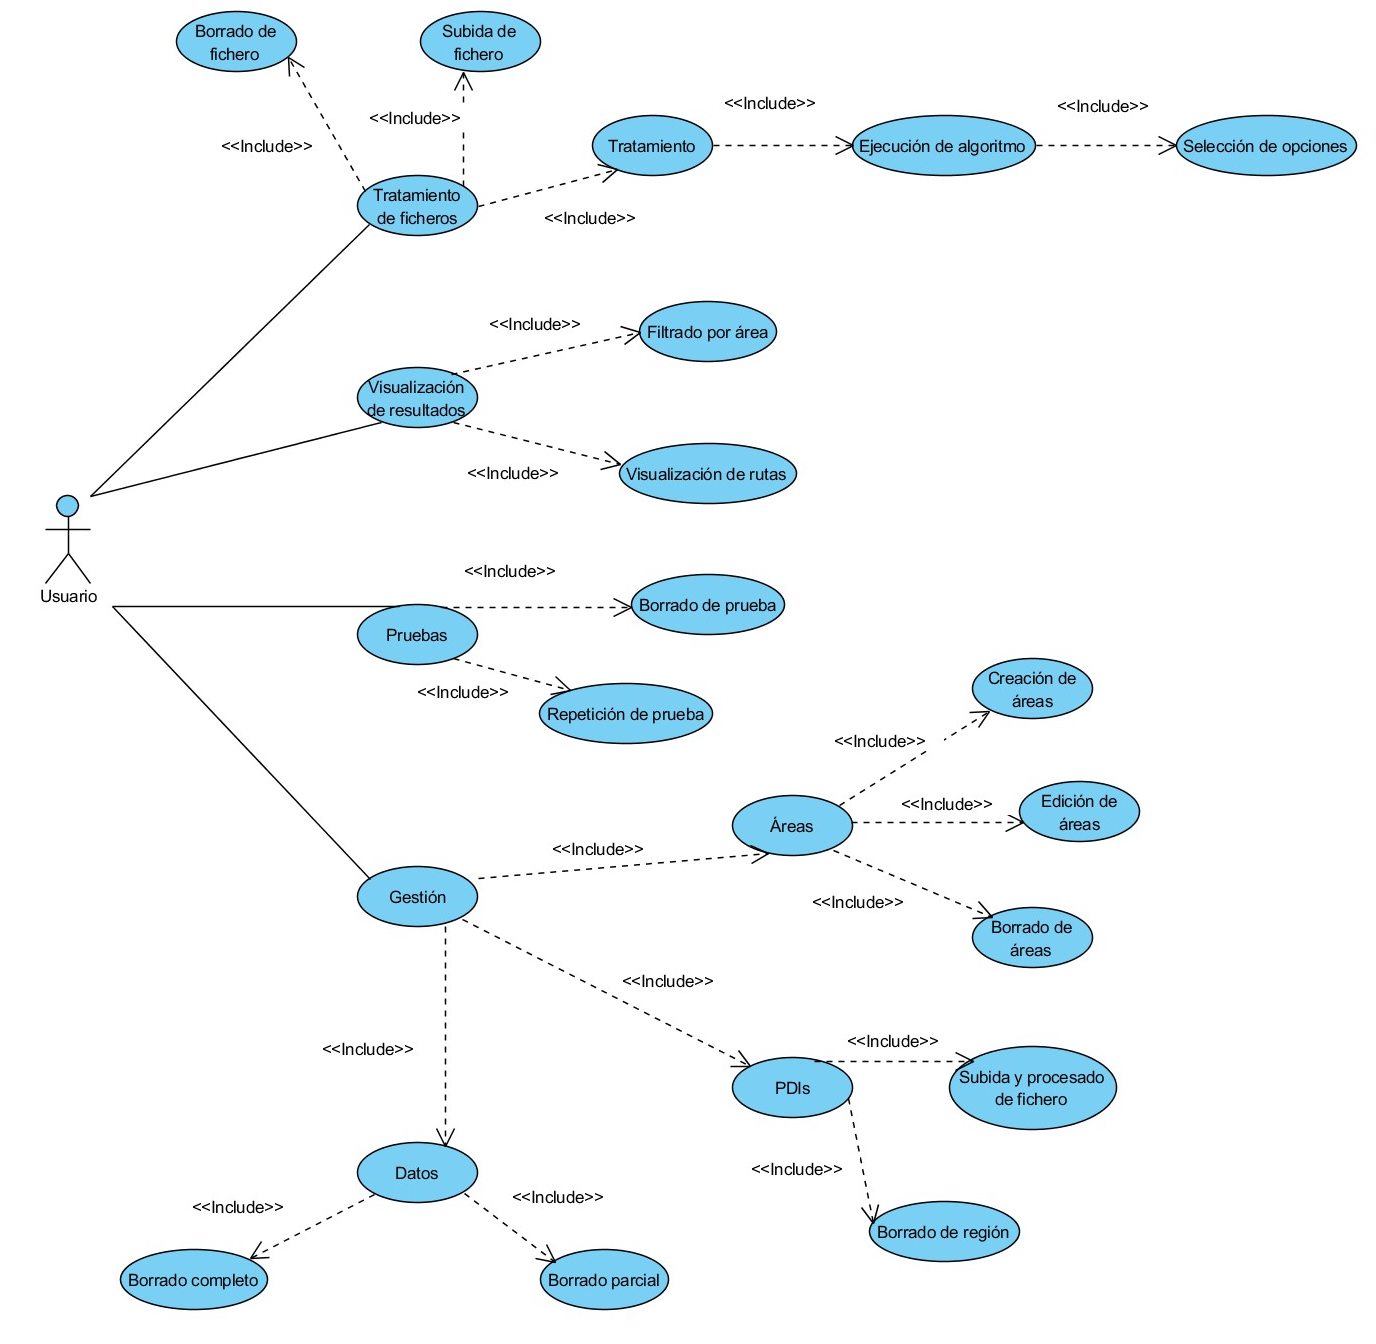
\includegraphics[width=0.8\textwidth]{../img/uml/casouso.png}
  \caption{Diagrama de casos de uso.}
  \label{casouso}
\end{figure}

\subsubsection{Actores}
Los actores son el conjunto de usuarios que pueden intervenir en el sistema desarrollado, en el caso  de esta aplicación web solo se contará con un usuario estándar:

\begin{itemize}
	\item \textbf{Usuario:} el usuario será capaz de acceder a todas las páginas de la plataforma web.
\end{itemize}


\subsubsection{Casos de uso}
A continuación se muestran las tablas descriptivas de los casos de uso del sistema.
\begin{comment}
	FICHEROS -----------------
\end{comment}

\tablaSinColores{CU-1 Subida de ficheros}
{L{3.5cm} L{10cm}}
{2}
{Tabla CU-01}
{\textbf{CU-01} & \textbf{Subida de ficheros} \\}
{\textbf{Versión} 				& 1.0\\ 
 \textbf{Autor} 				& David Moreno del Hoyo\\
 \textbf{Requisitos asociados} 	& RF-1, RF-2 \\
 \textbf{Descripción} 			& 
 La subida de ficheros implica la posibilidad de subir al servidor ficheros con rutas para ser analizados.\\
 \textbf{Precondiciones} 		& 
    \begin{itemize}
 		\item La Base de Datos está disponible.
 		\item Espacio en disco suficiente.
 	\end{itemize}
 \\
 \textbf{Acciones} 				& 
 	\begin{enumerate}
    	\item El usuario accede al sitio web.
    	\item El usuario selecciona un fichero mediante el formulario disponible.
    	\item El usuario clica sobre el botón \quotes{Enviar}.
    	\item El fichero es cargado en el sistema.
    	\item La página se refresca.
    \end{enumerate}
 \\
 
 \textbf{Postcondiciones} 		& 
    \begin{itemize}
 		\item El fichero será almacenado en el servidor.
 		\item El fichero será mostrado en la tabla de ficheros.
 	\end{itemize}
 \\
 \textbf{Excepciones} 			& 
 	\begin{itemize}
 		\item La base de datos no está disponible.
 	\end{itemize}
    
 \\
 \textbf{Importancia} 			& Alta\\}
 
  %%%%%%%%%%%%%%%%%%%%%%%%%%%%%%%%%%%%%%%%%%%%%%%%%%%%%



\tablaSinColores{CU-2 Borrado de ficheros}
{L{3.5cm} L{10cm}}
{2}
{Tabla CU-02}
{\textbf{CU-02} & \textbf{Borrado de ficheros} \\}
{\textbf{Versión} 				& 1.0\\ 
 \textbf{Autor} 				& David Moreno del Hoyo\\
 \textbf{Requisitos asociados} 	& RF-1, RF-2\\
 \textbf{Descripción} 			&  El borrado de ficheros permite borrar de forma total o parcial los ficheros del servidor.\\
 \textbf{Precondiciones} 		& 
    \begin{itemize}
 		\item La Base de Datos está disponible.
 		\item Existencia de ficheros.
 	\end{itemize}
 \\
 \textbf{Acciones} 				& 
 	\begin{enumerate}
    	\item El usuario accede al sitio web.
    	\item El usuario selecciona uno o varios ficheros existentes en el sistema.
    	\item El usuario clica sobre el botón \quotes{Eliminar}.
    	\item El fichero o ficheros son eliminados del sistema.
    	\item La página se refresca.
    \end{enumerate}
 \\
 
 \textbf{Postcondiciones} 		& 
    \begin{itemize}
 		\item El fichero se elimina.
 	\end{itemize}
 \\
 \textbf{Excepciones} 			& 
 	\begin{itemize}
 		\item La base de datos no está disponible.
 	\end{itemize}
    
 \\
 \textbf{Importancia} 			& Alta\\}
 
  %%%%%%%%%%%%%%%%%%%%%%%%%%%%%%%%%%%%%%%%%%%%%%%%%%%%%

\tablaSinColores{CU-3 Selección de opciones para el análisis de la ruta}
{L{3.5cm} L{10cm}}
{2}
{Tabla CU-03}
{\textbf{CU-03} & \textbf{Selección de opciones para el análisis de la ruta} \\}
{\textbf{Versión} 				& 1.0\\ 
 \textbf{Autor} 				& David Moreno del Hoyo\\
 \textbf{Requisitos asociados} 	& RF-2, RF-3 \\
 \textbf{Descripción} 			&  Las opciones permiten modificar el comportamiento del algoritmo. \\
 \textbf{Precondiciones} 		& 
    \begin{itemize}
 		\item La Base de Datos está disponible.
 		\item Existencia de ficheros y selección de, al menos, uno.
 	\end{itemize}
 \\
 \textbf{Acciones} 				& 
 	\begin{enumerate}
		\item El usuario marca las opciones de área.
		\item El usuario marca las opciones de ruta.
		\item El usuario marca las opciones de parada.
		\item El usuario marca las opciones de PDIs.
		\item El usuario marca las opciones de almacenado.
    \end{enumerate}
 \\
 
 \textbf{Postcondiciones} 		& 
    \begin{itemize}
 		\item Se permite la ejecución del algoritmo.
 	\end{itemize}
 \\
 \textbf{Excepciones} 			& 
 	\begin{itemize}
 		\item La base de datos no está disponible.
 	\end{itemize}
    
 \\
 \textbf{Importancia} 			& Alta\\}
 
  %%%%%%%%%%%%%%%%%%%%%%%%%%%%%%%%%%%%%%%%%%%%%%%%%%%%%
  
\tablaSinColores{CU-4 Ejecución de algoritmo}
{L{3.5cm} L{10cm}}
{2}
{Tabla CU-04}
{\textbf{CU-04} & \textbf{Ejecución de algoritmo} \\}
{\textbf{Versión} 				& 1.0\\ 
 \textbf{Autor} 				& David Moreno del Hoyo\\
 \textbf{Requisitos asociados} 	& RF-2, RF-3 \\
 \textbf{Descripción} 			&  El algoritmo procesa los ficheros según las opciones marcadas por el usuario. \\
 \textbf{Precondiciones} 		& 
    \begin{itemize}
 		\item La Base de Datos está disponible.
 		\item Existencia de ficheros y selección de, al menos, uno.
 		\item Selección de opciones.
 	\end{itemize}
 \\
 \textbf{Acciones} 				& 
 	\begin{enumerate}
 		\item El usuario clica sobre el botón \quotes{Ejecutar}.
    \end{enumerate}
 \\
 
 \textbf{Postcondiciones} 		& 
    \begin{itemize}
 		\item El fichero se marca como analizado.
 		\item Se guardan los resultados de forma temporal o permanente.
 	\end{itemize}
 \\
 \textbf{Excepciones} 			& 
 	\begin{itemize}
 		\item La base de datos no está disponible.
 	\end{itemize}
    
 \\
 \textbf{Importancia} 			& Alta\\}
 
  %%%%%%%%%%%%%%%%%%%%%%%%%%%%%%%%%%%%%%%%%%%%%%%%%%%%%

\tablaSinColores{CU-5 Tratamiento de ficheros}
{L{3.5cm} L{10cm}}
{2}
{Tabla CU-05}
{\textbf{CU-05} & \textbf{Tratamiento de ficheros} \\}
{\textbf{Versión} 				& 1.0\\ 
 \textbf{Autor} 				& David Moreno del Hoyo\\
 \textbf{Requisitos asociados} 	& RF-1, RF-3\\
 \textbf{Descripción} 			&  El tratamiento de ficheros permite seleccionarlos para ser analizados por el algoritmo.\\
 \textbf{Precondiciones} 		& 
    \begin{itemize}
 		\item La Base de Datos está disponible.
 		\item Existencia de ficheros.
 	\end{itemize}
 \\
 \textbf{Acciones} 				& 
 	\begin{enumerate}
    	\item El usuario accede al sitio web.
    	\item El usuario selecciona uno o varios ficheros existentes en el sistema.
    	\item El usuario clica sobre el botón \quotes{Procesar}.
    	\item El usuario selecciona las opciones de procesado del algoritmo.
    	\item El usuario clica sobre el botón \quotes{Procesar}.
    	\item El algoritmo procesa los ficheros.
    	\item La página se refresca con el resultado del proceso.
    \end{enumerate}
 \\
 
 \textbf{Postcondiciones} 		& 
    \begin{itemize}
 		\item La Base de Datos del sistema se actualiza con los datos obtenidos.
 		\item El fichero se marca como analizado.
 	\end{itemize}
 \\
 \textbf{Excepciones} 			& 
 	\begin{itemize}
 		\item La base de datos no está disponible.
 	\end{itemize}
    
 \\
 \textbf{Importancia} 			& Alta\\}
 
  %%%%%%%%%%%%%%%%%%%%%%%%%%%%%%%%%%%%%%%%%%%%%%%%%%%%%

\begin{comment}
	VISUALIZACIÓN DE RESULTADOS -----------------
\end{comment}



\tablaSinColores{CU-6 Visualización de resultados}
{L{3.5cm} L{10cm}}
{2}
{Tabla CU-06}
{\textbf{CU-06} & \textbf{Visualización de resultados} \\}
{\textbf{Versión} 				& 1.0\\ 
 \textbf{Autor} 				& David Moreno del Hoyo\\
 \textbf{Requisitos asociados} 	& RF-4, RF-6\\
 \textbf{Descripción} 			&  Se permite visualizar los resultados de las ejecuciones de las pruebas. \\
 \textbf{Precondiciones} 		& 
    \begin{itemize}
 		\item La Base de Datos está disponible.
 		\item Existencia de pruebas realizadas.
 	\end{itemize}
 \\
 \textbf{Acciones} 				& 
 	\begin{enumerate}
    	\item El usuario accede al sitio web.
    \end{enumerate}
 \\
 
 \textbf{Postcondiciones} 		& 
    \begin{itemize}
 		\item La página se actualiza con las áreas y rutas existentes.
 	\end{itemize}
 \\
 \textbf{Excepciones} 			& 
 	\begin{itemize}
 		\item La base de datos no está disponible.
 	\end{itemize}
    
 \\
 \textbf{Importancia} 			& Alta\\}
 
  %%%%%%%%%%%%%%%%%%%%%%%%%%%%%%%%%%%%%%%%%%%%%%%%%%%%%


\tablaSinColores{CU-7 Filtrado por área}
{L{3.5cm} L{10cm}}
{2}
{Tabla CU-07}
{\textbf{CU-07} & \textbf{Filtrado por área} \\}
{\textbf{Versión} 				& 1.0\\ 
 \textbf{Autor} 				& David Moreno del Hoyo\\
 \textbf{Requisitos asociados} 	& RF-3, RF-4\\
 \textbf{Descripción} 			&  Se permite filtrar las rutas por área. \\
 \textbf{Precondiciones} 		& 
    \begin{itemize}
 		\item La Base de Datos está disponible.
 		\item Existencia de pruebas anteriores.
 	\end{itemize}
 \\
 \textbf{Acciones} 				& 
 	\begin{enumerate}
    	\item El usuario accede al sitio web.
    	\item El usuario hace uso del filtro de área.
    	\begin{itemize}
    		\item Selecciona un área o.
    		\item Selecciona una zona del mapa o.
    		\item Introduce los datos del área de forma manual.
    	\end{itemize}
    \end{enumerate}
 \\
 
 \textbf{Postcondiciones} 		& 
    \begin{itemize}
 		\item La página se actualiza con las áreas y rutas existentes.
 	\end{itemize}
 \\
 \textbf{Excepciones} 			& 
 	\begin{itemize}
 		\item La base de datos no está disponible.
 	\end{itemize}
    
 \\
 \textbf{Importancia} 			& Alta\\}
 
  %%%%%%%%%%%%%%%%%%%%%%%%%%%%%%%%%%%%%%%%%%%%%%%%%%%%%


\tablaSinColores{CU-8 Visualización de rutas}
{L{3.5cm} L{10cm}}
{2}
{Tabla CU-08}
{\textbf{CU-08} & \textbf{Visualización de rutas} \\}
{\textbf{Versión} 				& 1.0\\ 
 \textbf{Autor} 				& David Moreno del Hoyo\\
 \textbf{Requisitos asociados} 	& RF-3, RF-4, RF-5\\
 \textbf{Descripción} 			& Se permite visualizar las rutas seleccionadas. \\
 \textbf{Precondiciones} 		& 
    \begin{itemize}
 		\item La Base de Datos está disponible.
 		\item Existencia de pruebas anteriores.
 	\end{itemize}
 \\
 \textbf{Acciones} 				& 
 	\begin{enumerate}
    	\item El usuario accede al sitio web.
    	\item El usuario selecciona un área.
    	\item El usuario selecciona una o varias rutas.
    	\item El usuario clica en \quotes{Ver más}.
    \end{enumerate}
 \\
 
 \textbf{Postcondiciones} 		& 
    \begin{itemize}
 		\item La página se actualiza con las rutas marcadas.
 	\end{itemize}
 \\
 \textbf{Excepciones} 			& 
 	\begin{itemize}
 		\item La base de datos no está disponible.
 	\end{itemize}
    
 \\
 \textbf{Importancia} 			& Alta\\}
 
  %%%%%%%%%%%%%%%%%%%%%%%%%%%%%%%%%%%%%%%%%%%%%%%%%%%%%


\begin{comment}
	PRUEBAS -----------------
\end{comment}


\tablaSinColores{CU-9 Pruebas}
{L{3.5cm} L{10cm}}
{2}
{Tabla CU-09}
{\textbf{CU-09} & \textbf{Pruebas} \\}
{\textbf{Versión} 				& 1.0\\ 
 \textbf{Autor} 				& David Moreno del Hoyo\\
 \textbf{Requisitos asociados} 	& RF-4\\
 \textbf{Descripción} 			& Permite al usuario acceder a las pruebas realizadas con anterioridad. La tabla que contiene la página permitirá al usuario ver las opciones seleccionadas por cada ejecución. \\
 \textbf{Precondiciones} 		& 
    \begin{itemize}
 		\item La Base de Datos está disponible.
 		\item Existencia de pruebas anteriores.
 	\end{itemize}
 \\
 \textbf{Acciones} 				& 
 	\begin{enumerate}
    	\item El usuario accede al sitio web.
    \end{enumerate}
 \\
 
 \textbf{Postcondiciones} 		& 
    \begin{itemize}
 		\item La página muestra las pruebas existentes en una tabla.
 	\end{itemize}
 \\
 \textbf{Excepciones} 			& 
 	\begin{itemize}
 		\item La base de datos no está disponible.
 	\end{itemize}
    
 \\
 \textbf{Importancia} 			& Alta\\}
 
  %%%%%%%%%%%%%%%%%%%%%%%%%%%%%%%%%%%%%%%%%%%%%%%%%%%%%
  
  \tablaSinColores{CU-10 Borrado de pruebas}
{L{3.5cm} L{10cm}}
{2}
{Tabla CU-10}
{\textbf{CU-10} & \textbf{Borrado de pruebas} \\}
{\textbf{Versión} 				& 1.0\\ 
 \textbf{Autor} 				& David Moreno del Hoyo\\
 \textbf{Requisitos asociados} 	& RF-4\\
 \textbf{Descripción} 			&  Se permite el borrado de una de las pruebas realizadas. Se eliminará del sistema y la tabla de pruebas será actualizada. \\
 \textbf{Precondiciones} 		& 
    \begin{itemize}
 		\item La Base de Datos está disponible.
 		\item Existencia de pruebas anteriores.
 	\end{itemize}
 \\
 \textbf{Acciones} 				& 
 	\begin{enumerate}
    	\item El usuario accede al sitio web.
    	\begin{itemize}
    	\item El usuario clica sobre el botón \quotes{Eliminar} de una de las rutas o.
    	\item El usuario clica sobre el botón \quotes{Eliminar todas las pruebas}.
    	\end{itemize}

    \end{enumerate}
 \\
 
 \textbf{Postcondiciones} 		& 
    \begin{itemize}
 		\item La página se actualiza con las pruebas existentes en la tabla.
 	\end{itemize}
 \\
 \textbf{Excepciones} 			& 
 	\begin{itemize}
 		\item La base de datos no está disponible.
 	\end{itemize}
    
 \\
 \textbf{Importancia} 			& Alta\\}
 
  %%%%%%%%%%%%%%%%%%%%%%%%%%%%%%%%%%%%%%%%%%%%%%%%%%%%%
  
  \tablaSinColores{CU-11 Repetición de prueba}
{L{3.5cm} L{10cm}}
{2}
{Tabla CU-11}
{\textbf{CU-11} & \textbf{Repetición de prueba} \\}
{\textbf{Versión} 				& 1.0\\ 
 \textbf{Autor} 				& David Moreno del Hoyo\\
 \textbf{Requisitos asociados} 	& RF-2, RF-3\\
 \textbf{Descripción} 			&  Permite al usuario repetir una de las pruebas con los datos de la misma o modificándolos según su criterio. \\
 \textbf{Precondiciones} 		& 
    \begin{itemize}
 		\item La Base de Datos está disponible.
 		\item Existencia de pruebas anteriores.
 	\end{itemize}
 \\
 \textbf{Acciones} 				& 
 	\begin{enumerate}
    	\item El usuario accede al sitio web.
    	\item El usuario selecciona una prueba y clica sobre el botón \quotes{Repetir}.
    	\item La página redirecciona al usuario a la sección de ejecución del algoritmo.
    \end{enumerate}
 \\
 
 \textbf{Postcondiciones} 		& 
    \begin{itemize}
 		\item La página de opciones del algoritmo se carga con los datos de la prueba seleccionada.
 	\end{itemize}
 \\
 \textbf{Excepciones} 			& 
 	\begin{itemize}
 		\item La base de datos no está disponible.
 	\end{itemize}
    
 \\
 \textbf{Importancia} 			& Alta\\}
 
  %%%%%%%%%%%%%%%%%%%%%%%%%%%%%%%%%%%%%%%%%%%%%%%%%%%%%


\begin{comment}
	GESTIÓN -----------------
\end{comment}


\tablaSinColores{CU-12 Gestión}
{L{3.5cm} L{10cm}}
{2}
{Tabla CU-12}
{\textbf{CU-12} & \textbf{Gestión} \\}
{\textbf{Versión} 				& 1.0\\ 
 \textbf{Autor} 				& David Moreno del Hoyo\\
 \textbf{Requisitos asociados} 	& RF-3\\
 \textbf{Descripción} 			&  La página de gestión permite al usuario seleccionar una de las tres opciones mostradas en dicha página. \\
 \textbf{Precondiciones} 		& 
    \begin{itemize}
 		\item La Base de Datos está disponible.
 	\end{itemize}
 \\
 \textbf{Acciones} 				& 
 	\begin{enumerate}
    	\item El usuario accede al sitio web.
    	\item El usuario selecciona una de las opciones que muestra la página de gestión.
    \end{enumerate}
 \\
 
 \textbf{Postcondiciones} 		& 
    \begin{itemize}
 		\item Se carga la página seleccionada.
 	\end{itemize}
 \\
 \textbf{Excepciones} 			& 
 	\begin{itemize}
 		\item La base de datos no está disponible.
 	\end{itemize}
    
 \\
 \textbf{Importancia} 			& Alta\\}

  %%%%%%%%%%%%%%%%%%%%%%%%%%%%%%%%%%%%%%%%%%%%%%%%%%%%%

\begin{comment}
	GESTIÓN - > DATOS -----------------
\end{comment}

\tablaSinColores{CU-13 Gestión de Datos}
{L{3.5cm} L{10cm}}
{2}
{Tabla CU-13}
{\textbf{CU-13} & \textbf{Gestión de Datos} \\}
{\textbf{Versión} 				& 1.0\\ 
 \textbf{Autor} 				& David Moreno del Hoyo\\
 \textbf{Requisitos asociados} 	& RF-3, RF-4\\
 \textbf{Descripción} 			&  La página de gestión de datos muestra las opciones de borrado de datos. \\
 \textbf{Precondiciones} 		& 
    \begin{itemize}
 		\item La Base de Datos está disponible.
 	\end{itemize}
 \\
 \textbf{Acciones} 				& 
 	\begin{enumerate}
    	\item El usuario accede al sitio web.
    \end{enumerate}
 \\
 
 \textbf{Postcondiciones} 		& 
    \begin{itemize}
 		\item Se carga la página seleccionada.
 	\end{itemize}
 \\
 \textbf{Excepciones} 			& 
 	\begin{itemize}
 		\item La base de datos no está disponible.
 	\end{itemize}
    
 \\
 \textbf{Importancia} 			& Alta\\}

  %%%%%%%%%%%%%%%%%%%%%%%%%%%%%%%%%%%%%%%%%%%%%%%%%%%%%


\tablaSinColores{CU-14 Borrado completo de datos}
{L{3.5cm} L{10cm}}
{2}
{Tabla CU-14}
{\textbf{CU-14} & \textbf{Borrado completo de datos} \\}
{\textbf{Versión} 				& 1.0\\ 
 \textbf{Autor} 				& David Moreno del Hoyo\\
 \textbf{Requisitos asociados} 	& RF-3, RF-4\\
 \textbf{Descripción} 			& En la página de gestión de datos se permite el borrado total de los mismos. \\
 \textbf{Precondiciones} 		& 
    \begin{itemize}
 		\item La Base de Datos está disponible.
 	\end{itemize}
 \\
 \textbf{Acciones} 				& 
 	\begin{enumerate}
    	\item El usuario accede al sitio web.
    	\item El usuario selecciona la opción de Borrado completo.
    	\item El usuario clica sobre \quotes{Eliminar}.
    	\item La página muestra un aviso de borrado.
    	\item El usuario acepta el aviso.
    \end{enumerate}
 \\
 
 \textbf{Postcondiciones} 		& 
    \begin{itemize}
 		\item Los datos son eliminados.
 		\item Se muestra un aviso de borrado completado.
 	\end{itemize}
 \\
 \textbf{Excepciones} 			& 
 	\begin{itemize}
 		\item La base de datos no está disponible.
 	\end{itemize}
    
 \\
 \textbf{Importancia} 			& Alta\\}
 
   %%%%%%%%%%%%%%%%%%%%%%%%%%%%%%%%%%%%%%%%%%%%%%%%%%%%%
 
 
 \tablaSinColores{CU-15 Borrado parcial de datos}
{L{3.5cm} L{10cm}}
{2}
{Tabla CU-15}
{\textbf{CU-15} & \textbf{Borrado parcial de datos} \\}
{\textbf{Versión} 				& 1.0\\ 
 \textbf{Autor} 				& David Moreno del Hoyo\\
 \textbf{Requisitos asociados} 	& RF-3, RF-4\\
 \textbf{Descripción} 			& La página de gestión de datos permite un borrado parcial de los mismos. \\
 \textbf{Precondiciones} 		& 
    \begin{itemize}
 		\item La Base de Datos está disponible.
 	\end{itemize}
 \\
 \textbf{Acciones} 				& 
 	\begin{enumerate}
    	\item El usuario accede al sitio web.
    	\item El usuario selecciona la opción de Borrado completo.
    	\item El usuario clica sobre \quotes{Eliminar PDIs}.
    	\item La página muestra un aviso de borrado.
    	\item El usuario acepta el aviso.
    \end{enumerate}
 \\
 
 \textbf{Postcondiciones} 		& 
    \begin{itemize}
 		\item Los datos son eliminados.
 		\item Se muestra un aviso de borrado completado.
 	\end{itemize}
 \\
 \textbf{Excepciones} 			& 
 	\begin{itemize}
 		\item La base de datos no está disponible.
 	\end{itemize}
    
 \\
 \textbf{Importancia} 			& Alta\\}

  %%%%%%%%%%%%%%%%%%%%%%%%%%%%%%%%%%%%%%%%%%%%%%%%%%%%%





\begin{comment}
	GESTIÓN - > PDIs -----------------
\end{comment}


 \tablaSinColores{CU-16 Gestión de PDIs}
{L{3.5cm} L{10cm}}
{2}
{Tabla CU-16}
{\textbf{CU-16} & \textbf{Gestión de PDIs} \\}
{\textbf{Versión} 				& 1.0\\ 
 \textbf{Autor} 				& David Moreno del Hoyo\\
 \textbf{Requisitos asociados} 	& RF-1, RF-4\\
 \textbf{Descripción} 			& La página de gestión de PDIs permite visualizar y mantener los PDIs o subir nuevos PDIs al servidor. \\
 \textbf{Precondiciones} 		& 
    \begin{itemize}
 		\item La Base de Datos está disponible.
 	\end{itemize}
 \\
 \textbf{Acciones} 				& 
 	\begin{enumerate}
    	\item El usuario accede al sitio web.
    \end{enumerate}
 \\
 
 \textbf{Postcondiciones} 		& 
    \begin{itemize}
 		\item Se muestran los PDIs actuales en una tabla dividida en regiones.
 	\end{itemize}
 \\
 \textbf{Excepciones} 			& 
 	\begin{itemize}
 		\item La base de datos no está disponible.
 	\end{itemize}
    
 \\
 \textbf{Importancia} 			& Alta\\}

  %%%%%%%%%%%%%%%%%%%%%%%%%%%%%%%%%%%%%%%%%%%%%%%%%%%%%
  
  
   \tablaSinColores{CU-17 Subida y procesado de ficheros}
{L{3.5cm} L{10cm}}
{2}
{Tabla CU-17}
{\textbf{CU-17} & \textbf{Subida y procesado de ficheros} \\}
{\textbf{Versión} 				& 1.0\\ 
 \textbf{Autor} 				& David Moreno del Hoyo\\
 \textbf{Requisitos asociados} 	& RF-1\\
 \textbf{Descripción} 			& El formulario de subida permite subir y procesar un fichero de PDIs. \\
 \textbf{Precondiciones} 		& 
    \begin{itemize}
 		\item La Base de Datos está disponible.		
 	\end{itemize}
 \\
 \textbf{Acciones} 				& 
 	\begin{enumerate}
 		\item El usuario accede al sitio web.
    	\item Selecciona de un fichero en el área de gestión de PDIs.
    	\item El usuario indica una región.
    	\item El usuario clica en \quotes{Enviar}.
    	\item La página muestra el proceso de subida.
    \end{enumerate}
 \\
 
 \textbf{Postcondiciones} 		& 
    \begin{itemize}
 		\item La página se recarga con los datos subidos.
 	\end{itemize}
 \\
 \textbf{Excepciones} 			& 
 	\begin{itemize}
 		\item La base de datos no está disponible.
 	\end{itemize}
    
 \\
 \textbf{Importancia} 			& Alta\\}

  %%%%%%%%%%%%%%%%%%%%%%%%%%%%%%%%%%%%%%%%%%%%%%%%%%%%%
  
  
   \tablaSinColores{CU-18 Borrado de región}
{L{3.5cm} L{10cm}}
{2}
{Tabla CU-18}
{\textbf{CU-18} & \textbf{Borrado de región} \\}
{\textbf{Versión} 				& 1.0\\ 
 \textbf{Autor} 				& David Moreno del Hoyo\\
 \textbf{Requisitos asociados} 	& RF-3, RF-4\\
 \textbf{Descripción} 			& La página de gestión de PDIs permite eliminar la región a las que un conjunto de PDIs está asociado. \\
 \textbf{Precondiciones} 		& 
    \begin{itemize}
 		\item La Base de Datos está disponible.
 		\item Existencia de PDIs y regiones.
 	\end{itemize}
 \\
 \textbf{Acciones} 				& 
 	\begin{enumerate}
    	\item El usuario accede al sitio web.
    	\item El usuario accede a la página de gestión.
    	\item El usuario clica sobre el botón de \quotes{Eliminar} de la región.
    \end{enumerate}
 \\
 
 \textbf{Postcondiciones} 		& 
    \begin{itemize}
 		\item Se actualiza la Base de Datos y la tabla con las regiones restantes.
 	\end{itemize}
 \\
 \textbf{Excepciones} 			& 
 	\begin{itemize}
 		\item La base de datos no está disponible.
 	\end{itemize}
    
 \\
 \textbf{Importancia} 			& Alta\\}

  %%%%%%%%%%%%%%%%%%%%%%%%%%%%%%%%%%%%%%%%%%%%%%%%%%%%%  
  
  
\begin{comment}
	GESTIÓN - > ÁREAS -----------------
\end{comment}


   \tablaSinColores{CU-19 Áreas}
{L{3.5cm} L{10cm}}
{2}
{Tabla CU-19}
{\textbf{CU-19} & \textbf{Áreas} \\}
{\textbf{Versión} 				& 1.0\\ 
 \textbf{Autor} 				& David Moreno del Hoyo\\
 \textbf{Requisitos asociados} 	& RF-3, RF-4\\
 \textbf{Descripción} 			& La página de áreas permite mantener las áreas del sistema así como crear nuevas áreas. \\
 \textbf{Precondiciones} 		& 
    \begin{itemize}
 		\item La Base de Datos está disponible.
 	\end{itemize}
 \\
 \textbf{Acciones} 				& 
 	\begin{enumerate}
    	\item El usuario accede al sitio web.
    \end{enumerate}
 \\
 
 \textbf{Postcondiciones} 		& 
    \begin{itemize}
 		\item Se actualiza la página con las áreas disponibles en una tabla.
 	\end{itemize}
 \\
 \textbf{Excepciones} 			& 
 	\begin{itemize}
 		\item La base de datos no está disponible.
 	\end{itemize}
    
 \\
 \textbf{Importancia} 			& Alta\\}

  %%%%%%%%%%%%%%%%%%%%%%%%%%%%%%%%%%%%%%%%%%%%%%%%%%%%%  
  
     \tablaSinColores{CU-20 Creación de áreas}
{L{3.5cm} L{10cm}}
{2}
{Tabla CU-20}
{\textbf{CU-20} & \textbf{Creación de áreas} \\}
{\textbf{Versión} 				& 1.0\\ 
 \textbf{Autor} 				& David Moreno del Hoyo\\
 \textbf{Requisitos asociados} 	& RF-3\\
 \textbf{Descripción} 			&  En la página de de áreas será posible crear una nueva área indicando los valores solicitados. \\
 \textbf{Precondiciones} 		& 
    \begin{itemize}
 		\item La Base de Datos está disponible.
 	\end{itemize}
 \\
 \textbf{Acciones} 				& 
 	\begin{enumerate}
    	\item El usuario accede al sitio web.
    	\item El usuario accede a la página de gestión.
    	\item El usuario clica sobre el botón de \quotes{Crear} área.
    	\item El usuario completa los campos del modal.
    	\item El usuario envía los datos.
    \end{enumerate}
 \\
 
 \textbf{Postcondiciones} 		& 
    \begin{itemize}
 		\item Se actualiza la Base de Datos.
 		\item La tabla se actualiza con los datos de las áreas.
 	\end{itemize}
 \\
 \textbf{Excepciones} 			& 
 	\begin{itemize}
 		\item La base de datos no está disponible.
 	\end{itemize}
    
 \\
 \textbf{Importancia} 			& Alta\\}

  %%%%%%%%%%%%%%%%%%%%%%%%%%%%%%%%%%%%%%%%%%%%%%%%%%%%%  
  
  
     \tablaSinColores{CU-21 Edición de áreas}
{L{3.5cm} L{10cm}}
{2}
{Tabla CU-21}
{\textbf{CU-21} & \textbf{Edición de áreas} \\}
{\textbf{Versión} 				& 1.0\\ 
 \textbf{Autor} 				& David Moreno del Hoyo\\
 \textbf{Requisitos asociados} 	& RF-3, RF-4\\
 \textbf{Descripción} 			& La página de áreas permite la edición de las áreas disponibles. \\
 \textbf{Precondiciones} 		& 
    \begin{itemize}
 		\item La Base de Datos está disponible.
 		\item Existencia de áreas.
 	\end{itemize}
 \\
 \textbf{Acciones} 				& 
 	\begin{enumerate}
    	\item El usuario accede al sitio web.
    	\item El usuario accede a la página de gestión.
    	\item El usuario clica sobre el botón de \quotes{Editar} del área.
    	\item El usuario completa el modal.
    	\item El usuario envía los datos.
    \end{enumerate}
 \\
 
 \textbf{Postcondiciones} 		& 
    \begin{itemize}
 		\item Se actualiza la Base de Datos y la tabla con las áreas disponibles.
 	\end{itemize}
 \\
 \textbf{Excepciones} 			& 
 	\begin{itemize}
 		\item La base de datos no está disponible.
 	\end{itemize}
    
 \\
 \textbf{Importancia} 			& Alta\\}

  %%%%%%%%%%%%%%%%%%%%%%%%%%%%%%%%%%%%%%%%%%%%%%%%%%%%%  
  
  
\tablaSinColores{CU-22 Borrado de áreas}
{L{3.5cm} L{10cm}}
{2}
{Tabla CU-22}
{\textbf{CU-22} & \textbf{Borrado de áreas} \\}
{\textbf{Versión} 				& 1.0\\ 
 \textbf{Autor} 				& David Moreno del Hoyo\\
 \textbf{Requisitos asociados} 	& RF-3, RF-4\\
 \textbf{Descripción} 			& La página de áreas permite el borrado de las áreas disponibles. \\
 \textbf{Precondiciones} 		& 
    \begin{itemize}
 		\item La Base de Datos está disponible.
 		\item Existencia de áreas.
 	\end{itemize}
 \\
 \textbf{Acciones} 				& 
 	\begin{enumerate}
    	\item El usuario accede al sitio web.
    	\item El usuario accede a la página de gestión.
    	\item El usuario clica sobre el botón de \quotes{Eliminar} del área correspondiente a la que desea eliminar.
    	\item El usuario acepta el aviso de borrado.
    \end{enumerate}
 \\
 
 \textbf{Postcondiciones} 		& 
    \begin{itemize}
 		\item La página se actualiza con los datos de las áreas restantes.
 	\end{itemize}
 \\
 \textbf{Excepciones} 			& 
 	\begin{itemize}
 		\item La base de datos no está disponible.
 	\end{itemize}
    
 \\
 \textbf{Importancia} 			& Alta\\}

  %%%%%%%%%%%%%%%%%%%%%%%%%%%%%%%%%%%%%%%%%%%%%%%%%%%%%  
\apendice{Especificación de diseño}

\section{Introducción}

\section{Diseño de datos}

\section{Diseño procedimental}

\section{Diseño arquitectónico}



\apendice{Documentación técnica de programación}

\section{Introducción}

\section{Estructura de directorios}

\section{Manual del programador}

\section{Compilación, instalación y ejecución del proyecto}

\section{Pruebas del sistema}

\section{Instalación de herramientas}

\subsection{Virtual Box}
El software de virtualización seleccionado ha sido Oracle VM Virtual Box en su versión 5.1. Este programa ha sido instalado sobre Windows 10, sistema que actúa como anfitrión.

La descarga de este software se puede realizar desde la siguiente dirección web: \url{https://www.virtualbox.org/wiki/Downloads}

\subsection{Ubuntu 16.04}
Como servidor se ha optado por la versión 16.04 de Ubuntu en su versión de escritorio. El sistema ha sido instalado sobre una máquina virtual haciendo uso del software mencionado en la sección anterior.

Para descargar una imagen de este Sistema Operativo se ha de acceder al siguiente enlace: \url{https://www.ubuntu.com/download/desktop}


\subsection{PostgreSQL 9.6 y PgAdmin 3}
PostgreSQL puede ser instalado en Ubuntu desde la consola de comandos. Para ello se han de seguir unos sencillos pasos.
El primer paso es actualizar el repositorio de Ubuntu mediante el siguiente comando sobre la consola:
\begin{lstlisting}
apt-get update
\end{lstlisting}
Ahora se puede comenzar la instalación de Postgres mediante la siguiente línea en la consola de comandos:
\begin{lstlisting}
apt-get install postgresql postgresql-contrib
\end{lstlisting}

Por último, si se desea hacer uso de PgAdmin 3, se podrá instalar mediante el siguiente comando:
\begin{lstlisting}
apt-get install pgadmin3
\end{lstlisting}

Una vez que Postgres ha sido instalado, se ha procedido a la configuración del usuario por defecto (``postgres'') y de la creación de un nuevo usuario ``rs'') para la adición de extensiones y creación de tablas necesarias.

\subsection{PostGIS}
PostGIS es una extensión espacial para las Bases de Datos PostgreSQL. Esta extensión añade soporte para objetos geográficos permitiendo consultas geográficas sobre la Base de Datos.
PostGIS se encuentra distribuido bajo licencia GNU General Public License.

Para instalar PostGIS sobre Ubuntu 16.04 se ha de teclear el siguiente comando:
\begin{lstlisting}
apt-get install postgis
\end{lstlisting}

Se puede obtener más información en la página web oficial de PostGIS: \url{http://www.postgis.net/}.

\subsection{QGIS}
QGIS es una herramienta de información geográfica libre y de código abierto que permite conexiones con PostgreSQL y visualización de los datos obtenidos sobre un mapa físico. También permite la obtención de información geográfica desde Open Street Maps. De esta forma se pueden superponer rutas/trazas obtenidas desde las tablas de la Base de Datos con los mapas de Open Street Maps.

Para instalar QGIS desde ubuntu se han de seguir los pasos mostrados a continuación:

El primer paso es añadir la ruta a los ficheros fuente de QGIS en el fichero ``sources.list'', para ello se puede abrir dicho fichero con el editor nano. Se encuentra en la siguiente ruta: ``etc/apt/''.
Las líneas a añadir son las siguientes y pueden ser incluidas en la parte final del fichero:
\begin{lstlisting}
deb http://qgis.org/debian xenial main
deb-src http://qgis.org/debian xenial main
\end{lstlisting}

Ahora se puede proceder a la instalación de QGIS sobre el Sistema Operativo:

\begin{lstlisting}
apt install qgis python-qgis qgis-plugin-grass
\end{lstlisting}

Una vez instalado, se puede configurar una conexión contra la Base de Datos instalada y configurada anteriormente. Para ello se ha de clicar en el icono de PostgreSQL ubicado en la columna central izquierda. Para ello se han de indicar valores como:

\begin{itemize}
\item \textbf{nombre:} valor que se dará al nombre de la conexión.
\item \textbf{servidor:} servidor contra el que se realizará la conexión. En este caso será el servidor local.
\item \textbf{ de datos:} la Base de Datos de la que serán obtenidos los datos.
\item \textbf{Autenticación:} nombre de usuario y contraseña  del usuario de PostgresQL usado para obtener la información.
\end{itemize}

Para obtener más información sobre QGIS se puede acceder al siguiente enlace: \url{http://www.qgis.org/es/docs/index.html}

\subsection{RouteConverter}
RouteConverter permite visualizar trazas en formato gpx sobre un mapa físico. Es un programa de uso sencillo y rápido.

Para poder usar RouteConverter en la máquina virtual se deberá acceder a la sección de descargas de su plataforma web: \url{http://www.routeconverter.de/downloads/es}. Se puede optar por la versión ''webstart`` o por la versión estable. Para ejecutar ambas se requiere contar con la versión actual de Java.

\section{Manual del usuario}



\subsection{Osmosis}
Osmosis permite extraer una ciudad concreta de un mapa con formato pbf. En el caso de este trabajo, se ha descargado el mapa de España y se ha extraído la ciudad de Burgos. A continuación, se muestran los pasos a dar para obtener un fichero osm.

\subsubsection{Descarga del mapa de España}
Accediendo a la web de descargas de Geofabrik será posible elegir el país cuyo mapa que se desea descargar. Clicando sobre el enlace mostrado en la Figura, se puede descargar el mapa de España en formato pbf.

\subsubsection{Extracción de una ciudad}
Para extraer una ciudad del plano que se acaba de descargar, se ha de abrir la consola del sistema y hacer uso del fichero "getMap.bat". Se necesitarán los siguientes argumentos (entre paréntesis las coordenadas que serán usadas en el caso de Burgos):
\begin{itemize}
	\item Nombre de la ciudad: con esta cadena nombraremos el fichero osm de salida.
	\item Coordenada GPS que indique la parte superior del segmento de mapa que se va a recortar (42.658202).
	\item Coordenada GPS que indique la parte derecha del segmento de mapa que se va a recortar (-3.12561).
	\item Coordenada GPS que indique la parte inferior del segmento de mapa que se va a recortar (41.364442).
	\item Coordenada GPS que indique la parte izquierda del segmento de mapa que se va a recortar (-4.3066641).
\end{itemize}

El comando a teclear constará de lo siguiente:
\begin{itemize}
	\item rb: permite leer el contenido del fichero pbf descargado.
	\item bb: permite extraer los datos indicados en la caja definida por las coordenadas geográficas indicadas a continuación.
	\item top: coordenada geográfica superior.
	\item right: coordenada geográfica derecha.
	\item bottom: coordenada geográfica inferior.
	\item left: coordenada geográfica izquierda.
	\item wx: permite escribir los datos en un fichero osm.
\end{itemize}

Para la ciudad de burgos, el comando será el mostrado en la Figura. Ejecutando el comando se obtendrá el fichero "Burgos.osm".


\subsection{Uso de RouteConverter}

Una vez que se cuenta con este software en el ordenador, se pueden generar rutas o cargar ficheros con rutas ya definidas. En este caso se mostrará cómo cargar los datos de una ruta almacenada en la Base de Datos de Open Street Maps.

El primer paso a dar es la descarga de la traza que se desee visualizar con este programa.

\subsubsection{Descarga de ficheros gpx}
La descarga se realizará desde la página web de Open Street Maps, concretamente en la sección "Trazas". En esta sección se verán las últimas trazas subidas por los usuarios. Eligiendo una traza aleatoria accedemos a la ventana mostrada en la  Figura. Clicando sobre "descargar" se descargará el fichero gpx.

Estos ficheros contendrán una estructura XML con una serie de puntos geográficos que conformarán la ruta seguida por el usuario. La ruta podrá ser identificada con su nombre, el nombre del autor y una breve descripción.

\subsubsection{Carga de ficheros en RouteConverter}

Para cargar la traza en el programa, primero se debe abrir el software y después clicar sobre Archivo, Abrir. En la ventana emergente se ha de seleccionar la traza y clicar sobre Aceptar. En este momento se mostrará la ruta que describe la traza descargada desde Open Street Maps como se aprecia en la Figura \ref{rutaLeonFormigal}.

\begin{figure}[h]
  \centering
    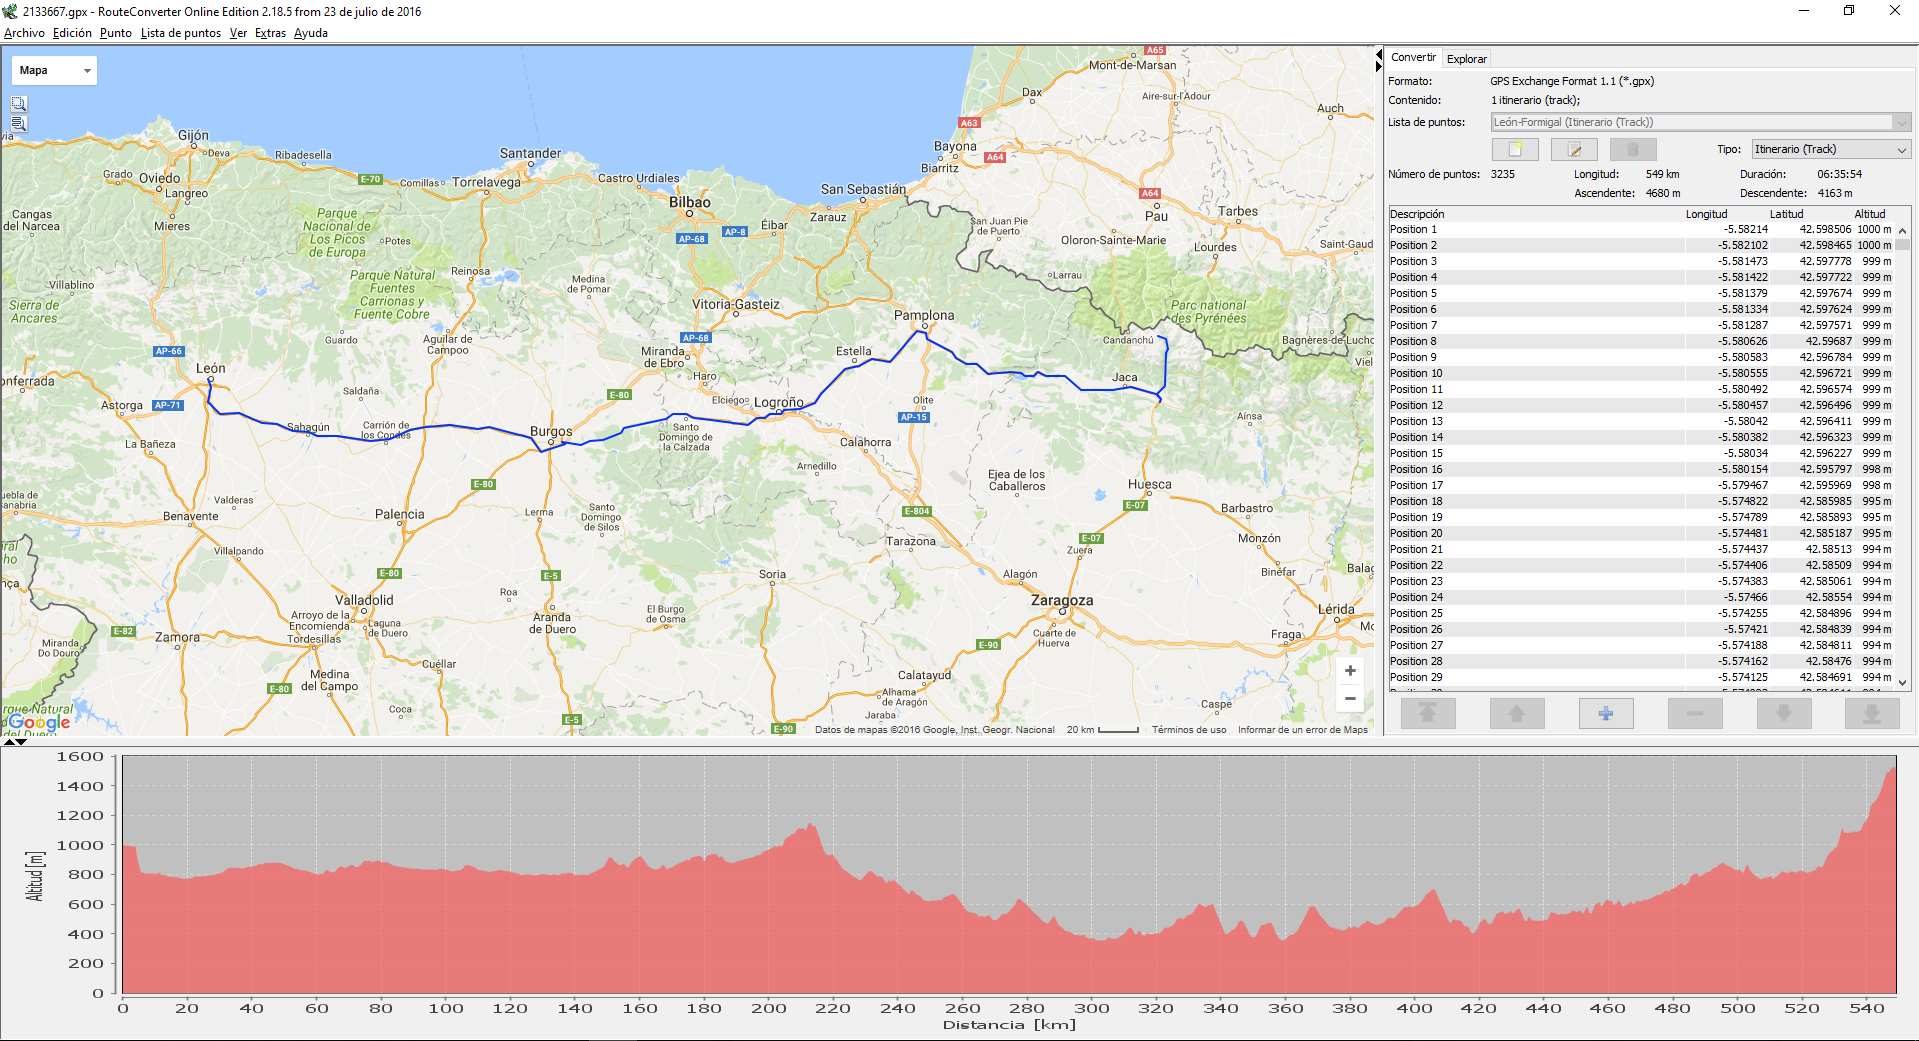
\includegraphics[width=0.8\textwidth]{../img/routeconverter/analisis_traza.png}
  \caption{Ruta desde León a Formigal}
  \label{rutaLeonFormigal}
\end{figure}

En la parte derecha de la ventana se pueden visualizar las rutas detectadas por el programa en el desplegable "Lista de puntos". En la parte inferior se listarán todos los puntos que conforman dicha lista como se ve en la Figura \ref{puntosGeograficos}.

\begin{figure}[h]
  \centering
    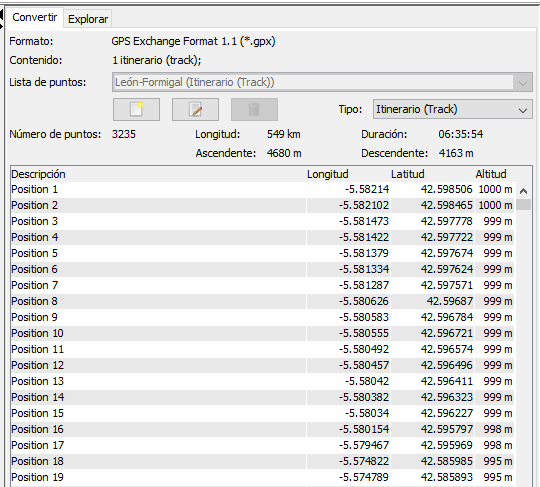
\includegraphics[width=0.6\textwidth]{../img/routeconverter/datos_traza.png}
  \caption{Ruta desde León a Formigal}
  \label{puntosGeograficos}
\end{figure}

Si la traza contiene elevaciones del terreno, se mostrará un perfil en la parte inferior.


\apendice{Documentación de usuario}

\section{Introducción}
En los siguientes apartados de este anexo se mostrará cuáles son los requisitos  y conocimientos mínimos necesarios para poder hacer uso de la plataforma web.

\section{Requisitos de usuarios}
Los requisitos mínimos son los siguientes:

\begin{itemize}
	\item Hardware: el recurso que puede limitar la experiencia de usuario es la cantidad de memoria RAM disponible, por ello, se recomienda contar con, al menos, 3 GiB de memoria RAM.
	\item Java: se ha de contar con el JRE de Java instalado y el servidor Glassfish para poder correr la plataforma de forma local.
	\item Base de Datos: se ha de contar con PostgreSQL como SGBD y su extensión PostGIS.
	\item Navegador: se ha de contar con un navegador web que soporte las últimas tecnologías, por ejemplo: Firefox o Chrome.
\end{itemize}

Cada sección de la plataforma web cuenta con una breve ayuda que permite al usuario desenvolverse con soltura desde el primer momento.

\section{Instalación}
La plataforma web no ha de instalarse ni seguir ningún proceso adicional. Para acceder a la misma se ha abrir un navegador y acceder al host local. Generalmente será de la siguiente forma:

\begin{lstlisting}[language=bash]
  http://localhost:8080/aplicacion\_web/
\end{lstlisting}

\section{Manual de usuario}
Esta sección describirá cómo es y cómo se usa la plataforma web. Se mostrarán las diferentes páginas que componen la plataforma web, las opciones de cada una de las mismas, etc.

En todas las páginas se mostrará un pequeño aviso en la parte superior si una prueba o la carga de ficheros de Puntos De Interés se encuentran activas. También mostrarán un botón de ayuda que desplegará un modal en el que se podrán leer los aspectos relevantes de uso de la página en concreto. La Figura \ref{ejealgo} muestra el aviso y la Figura \ref{botones} permite ver ambos botones.

\begin{figure}[h]
  \centering
    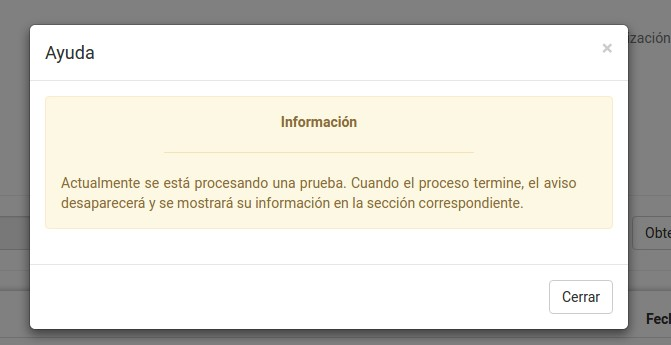
\includegraphics[width=0.6\textwidth]{../img/manualusuario/ejealgo.jpg}
  \caption{Ventana de aviso de un hilo en ejecución.}
  \label{ejealgo}
\end{figure}

\begin{figure}[h]
  \centering
    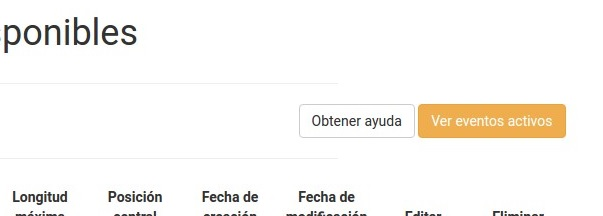
\includegraphics[width=0.6\textwidth]{../img/manualusuario/botones.jpg}
  \caption{Botones de ayuda e hilo en ejecución.}
  \label{botones}
\end{figure}

\subsection{Secciones de la plataforma web}

En este apartado se detallan las secciones con las que cuenta la plataforma web y cuáles son sus funciones:

\begin{itemize}
	\item Portada: la portada de la plataforma web muestra algunas de las características de la misma.
	\item Gestión de ficheros: la página de gestión de ficheros permite la subida, gestión y procesado de ficheros de rutas. Se permite la subida de ficheros de tipo csv. Estos ficheros serán mostrados en una tabla permitiendo su selección, procesado o eliminación de forma unitaria o conjunta.
	\item Visualización de resultados: la ventana de resultados cuenta con dos partes diferenciadas. A la izquierda se muestran tres formas diferentes de seleccionar las áreas disponibles en la Base de Datos. La primera forma consiste en seleccionar las áreas existentes, la segunda permite seleccionar un área dentro de un mapa, y la tercera consiste en introducir los valores de latitud y longitud manualmente. Una vez seleccionada una o varias áreas de la forma deseada por el usuario, el listado de rutas mostrado a la izquierda (segunda de las partes mencionadas) será actualizado con las rutas pertenecientes al área o a las áreas seleccionadas.
	\item Pruebas: esta página permite ver al usuario las pruebas que se han llevado a cabo del algoritmo de análisis de rutas. Se mostrará una tabla con los valores seleccionados en cada una de las ejecuciones del algoritmo y se permitirá su re ejecución, dejando al usuario la oportunidad de modificarlos o realizar la ejecución con los mismos valores.
	\item Gestión: en esta sección se encuentran las páginas de gestión de la plataforma web. Un primer apartado permite mantener las áreas que se encuentran en la Base de Datos, además de crear nuevas áreas.
\end{itemize}

\subsubsection{Portada}
La portada de esta plataforma muestra algunas imágenes y detalles de la misma que se consideran relevantes. Es, simplemente, un punto de entrada al sistema.

\subsubsection{Gestión de ficheros}
La página de gestión de ficheros se encuentra situada como segunda opción del menú principal de la plataforma web. Esta página permite al usuario una completa gestión de los ficheros subidos al servidor. Existe un formulario de subida que permite seleccionar ficheros únicos de tipo csv o ficheros comprimidos de tipo zip que, en su interior, contengan ficheros con extensión csv. La plataforma se encargará de la subida y eventual descompresión de los ficheros seleccionados por el usuario.

Un aviso indicará al usuario de que la subida ha sido satisfactoria o mostrará un error en caso de existir algún problema. Si la subida ha sido correcta, los ficheros serán mostrados en la tabla inmediatamente inferior al formulario. La Figura \ref{nofiles} muestra la página completamente vacía y la \ref{files} muestra el resultado de una primera carga de ficheros.

\begin{figure}[h]
  \centering
    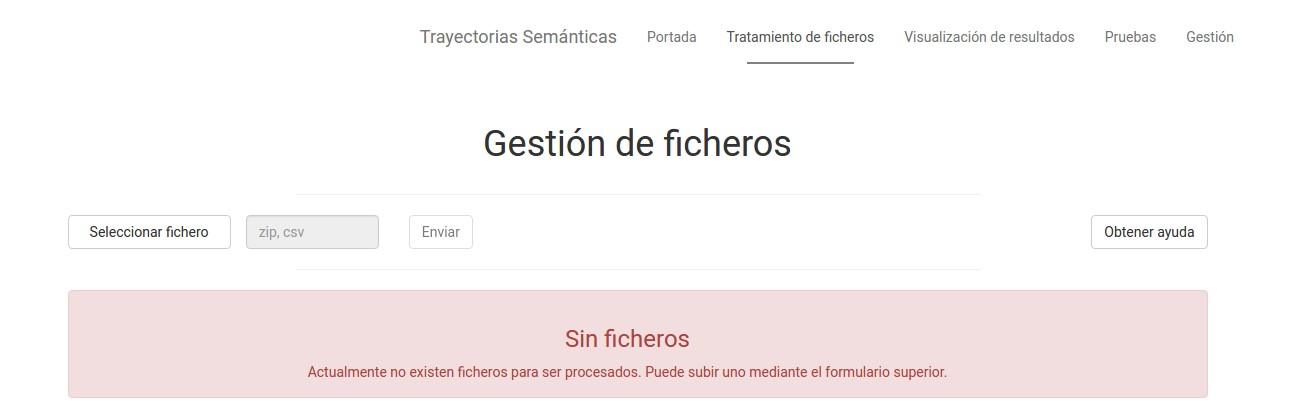
\includegraphics[width=0.6\textwidth]{../img/manualusuario/nofiles.jpg}
  \caption{Sin ficheros.}
  \label{nofiles}
\end{figure}

\begin{figure}[h]
  \centering
    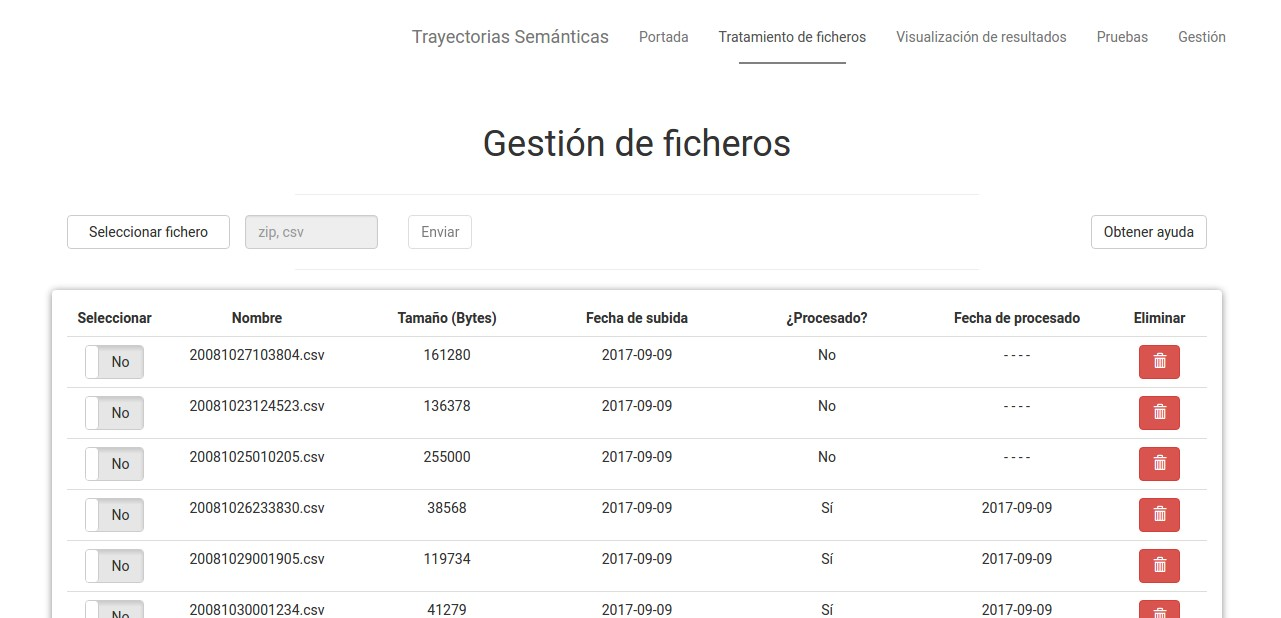
\includegraphics[width=0.6\textwidth]{../img/manualusuario/files.jpg}
  \caption{Carga de ficheros realizada correctamente.}
  \label{files}
\end{figure}

En caso de error, la Figura \ref{filerror} muestra el mensaje de error devuelto. El fichero no será subido.

\begin{figure}[h]
  \centering
    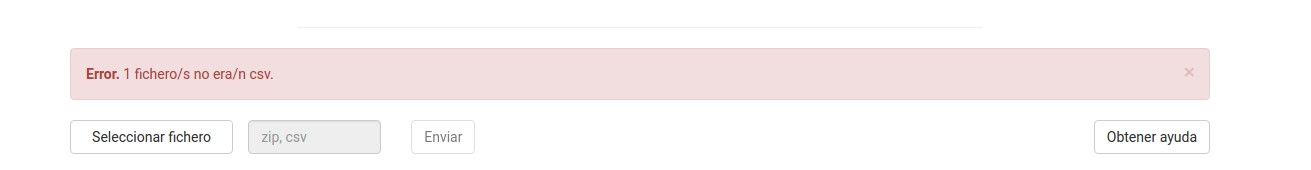
\includegraphics[width=0.6\textwidth]{../img/manualusuario/filerror.jpg}
  \caption{Error en la carga de ficheros.}
  \label{filerror}
\end{figure}

La tabla de ficheros muestra distinta información sobre los mismos. La siguiente lista muestra dicha información:

\begin{itemize}
	\item \textbf{Seleccionar:} cada fichero contará con un \textit{switch} que permitirá seleccionar el mismo para su procesado o borrado.
	\item \textbf{Nombre:} es el nombre del fichero con el que se subió a la plataforma. 
	\item \textbf{Tamaño:} es el tamaño en bytes que ocupa el fichero.
	\item \textbf{Fecha de subida:} la fecha en la que el fichero fue subida a la plataforma web.
	\item \textbf{Procesado:} indica al usuario si ya ha procesado ese fichero con anterioridad.
	\item \textbf{Fecha de procesado:} si así ha sido, se mostrará la fecha de procesado.
	\item \textbf{Eliminar:} botón que permite el borrado del fichero.
\end{itemize}

En la parte inferior de la tabla se encuentran tres botones adicionales:

\begin{itemize}
	\item \textbf{Seleccionar todos:} este botón permitirá seleccionar o liberar todos los ficheros de la tabla.
	\item \textbf{Eliminar ficheros seleccionados:} si se ha seleccionado alguno de los ficheros de la tabla, este botón se activará y permitirá borrar dichos ficheros.
	\item \textbf{Procesar los ficheros seleccionados:} una vez seleccionado alguno de los fichero y, clicando sobre este botón, se accederá a la página de opciones del algoritmo de análisis de rutas.
\end{itemize}

La Figura \ref{filetableend} muestra estos botones y su ubicación en la tabla.

\begin{figure}[h]
  \centering
    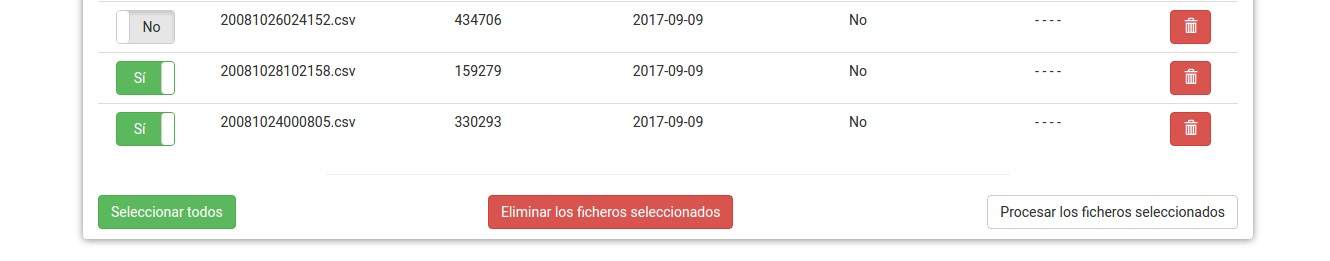
\includegraphics[width=0.6\textwidth]{../img/manualusuario/filetableend.jpg}
  \caption{Botones de la tabla de ficheros.}
  \label{filetableend}
\end{figure}

En caso de que una prueba se encuentre en ejecución, el botón de procesar ficheros quedará desactivado temporalmente hasta que la prueba termine, pudiéndose apreciar en la Figura \ref{pruebaeje}.

\begin{figure}[h]
  \centering
    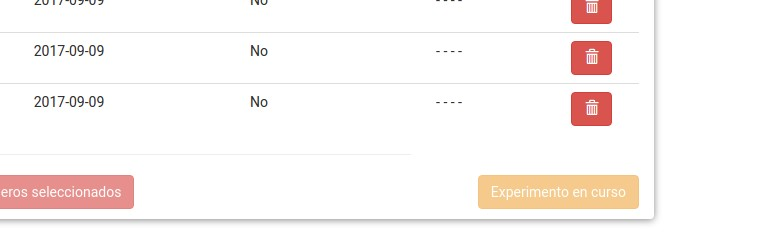
\includegraphics[width=0.6\textwidth]{../img/manualusuario/pruebaeje.jpg}
  \caption{Botón desactivado al encontrarse una prueba en ejecución.}
  \label{pruebaeje}
\end{figure}

\subsubsection{Opciones del algoritmo}
Una vez que el usuario ha seleccionado los ficheros que desea analizar, puede clicar en el botón \quotes{Procesar los ficheros seleccionados} y acceder a esta página de opciones.

En la parte izquierda de la ventana se podrán ver, en una tabla, los ficheros seleccionados. En la parte derecha se mostrarán las opciones disponibles antes de ejecutar el algoritmo. La Figura \ref{areaoption} permite ver, en la parte superior de los selectores, un pequeño indicador que señala la opción que actualmente aparece en pantalla. La Figura \ref{areaoption1} permite ver la segunda de las opciones, la selección de un área existente en la Base de Datos. Seleccionando esta última opción, se asignarán las rutas analizadas al área elegida.

\begin{figure}[h]
  \centering
    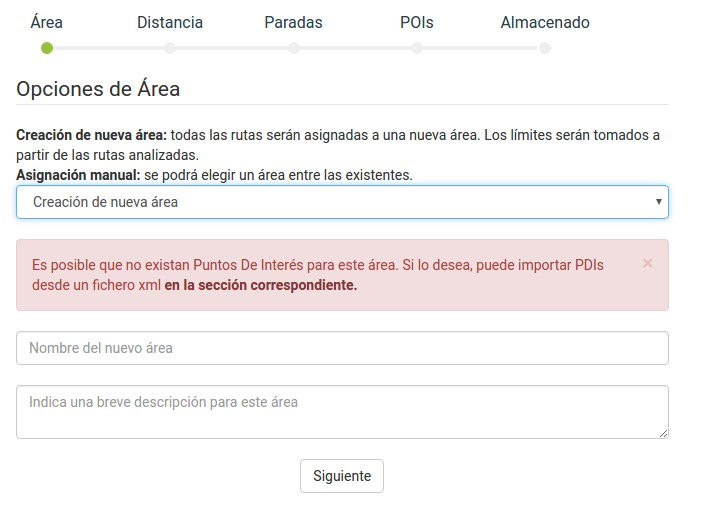
\includegraphics[width=0.6\textwidth]{../img/manualusuario/areaoption.jpg}
  \caption{Opción de creación de nueva área. Se indica en el aviso que pueden no existir Puntos De Interés para la zona que delimite esta nueva área.}
  \label{areaoption}
\end{figure}

\begin{figure}[h]
  \centering
    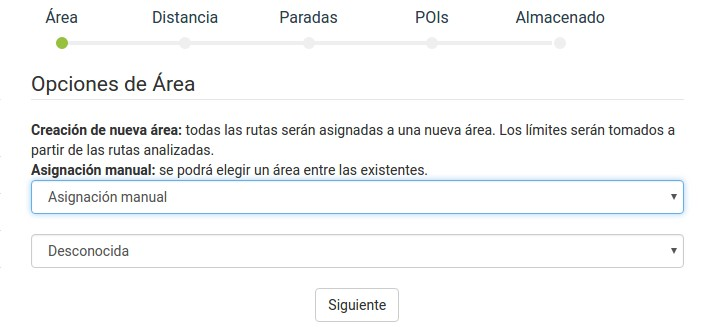
\includegraphics[width=0.6\textwidth]{../img/manualusuario/areaoption1.jpg}
  \caption{Opción de selección de un área existente.}
  \label{areaoption1}
\end{figure}

Clicando en siguiente se muestran las opciones para el análisis de la ruta. Como muestra la Figura \ref{rutaoption}, se cuentan con dos opciones, la primera de ellas permite seleccionar el corte de la ruta si entre dos posiciones de la misma se supera la distancia marcada como opción. También permite variar la mediana obtenida durante el análisis mediante el segundo de los valores, siendo este dato multiplicado por la cifra introducida por el usuario.

\begin{figure}[h]
  \centering
    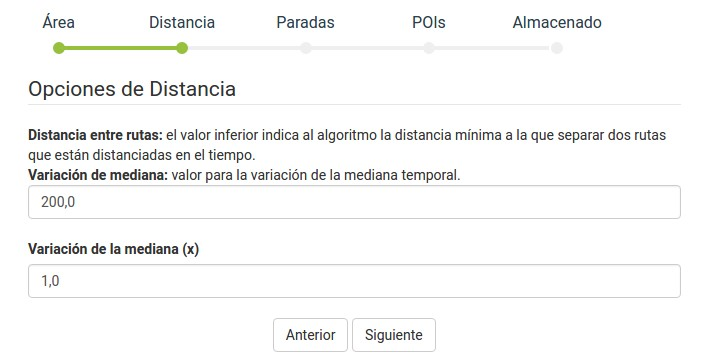
\includegraphics[width=0.6\textwidth]{../img/manualusuario/rutaoption.jpg}
  \caption{Opciones relativas al análisis de la ruta.}
  \label{rutaoption}
\end{figure}

La siguiente de las opciones permite al usuario decidir si quiere realizar una búsqueda de las paradas con las que puede contar la o las rutas de los ficheros seleccionados. Si desea realizar este análisis, la búsqueda de PDIs se activará. En caso contrario, la búsqueda de Puntos De Interés no estará disponible ya que los PDIs son asignados a las paradas encontradas en cada ruta.

La Figura \href{paradasi} permite ver las variables disponibles si se activa la búsqueda de paradas. La Figura \href{poisi} muestra lo propio con las posibilidades de búsqueda de Puntos De Interés. En caso de que no se deseen buscar paradas, el aviso que se aprecia en la Figura \ref{poino} será mostrado en la sección de PDIs.

\begin{figure}[h]
  \centering
    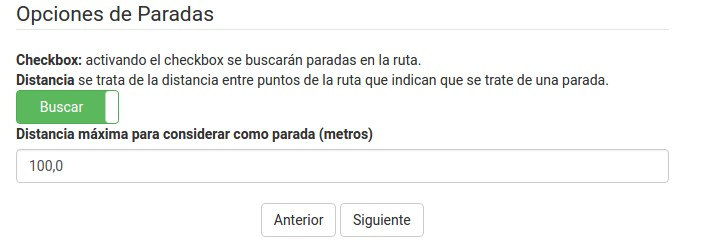
\includegraphics[width=0.6\textwidth]{../img/manualusuario/paradasi.jpg}
  \caption{Opciones de búsqueda de paradas.}
  \label{paradasi}
\end{figure}


\begin{figure}[h]
  \centering
    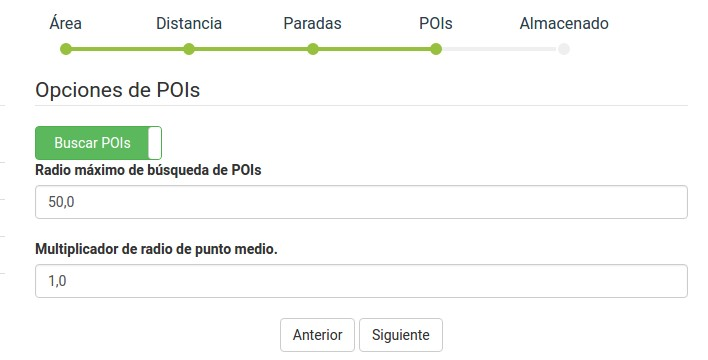
\includegraphics[width=0.6\textwidth]{../img/manualusuario/poisi.jpg}
  \caption{Opciones análisis de Puntos De Interés activas.}
  \label{poisi}
\end{figure}


\begin{figure}[h]
  \centering
    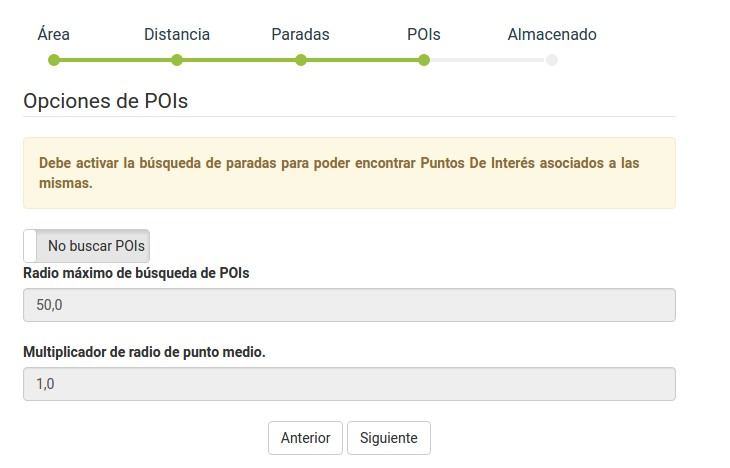
\includegraphics[width=0.6\textwidth]{../img/manualusuario/poino.jpg}
  \caption{Opciones análisis de Puntos De Interés desactivadas debido a que no se buscarán paradas.}
  \label{poino}
\end{figure}

La última de las opciones (Figura \ref{guardar}) que permite el algoritmo es el guardado de todos los datos en la Base de Datos del sistema. Estas opción permitirá almacenar de forma permanente los resultados obtenidos durante el análisis de ficheros. En caso de no desear guardar los datos, estos serán perdidos al cerrar el navegador.

\begin{figure}[h]
  \centering
    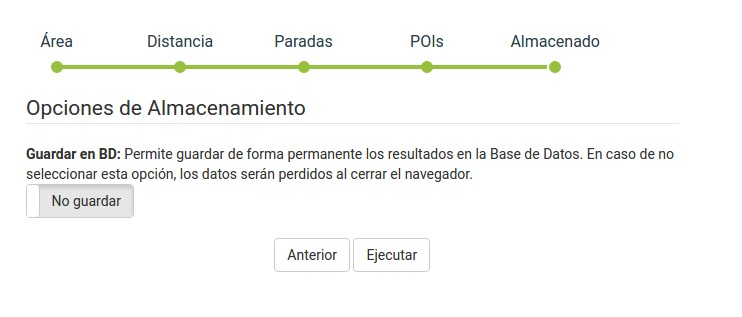
\includegraphics[width=0.6\textwidth]{../img/manualusuario/guardar.jpg}
  \caption{Opciones guardado, en la figura, la opción no está seleccionada.}
  \label{guardar}
\end{figure}

Una vez que el usuario está conforme con los datos elegidos para realizar el análisis puede clicar en el botón \quotes{Ejecutar} y comenzará el procesado de los ficheros. En caso de no estar seguro de los datos elegidos siempre puede volver atrás mediante el botón correspondiente y que se aprecia en las figuras mostradas.

La Figura \ref{enejecucion} muestra la página que se visualiza cuando una prueba se encuentra en ejecución. En esta página también se permite al usuario detener el proceso si estima que está siendo extremadamente largo y prefiere probar otros valores. En la parte inferior se puede ver un pequeño indicador del estado en el que se encuentra la ejecución del algoritmo de análisis.

\begin{figure}[h]
  \centering
    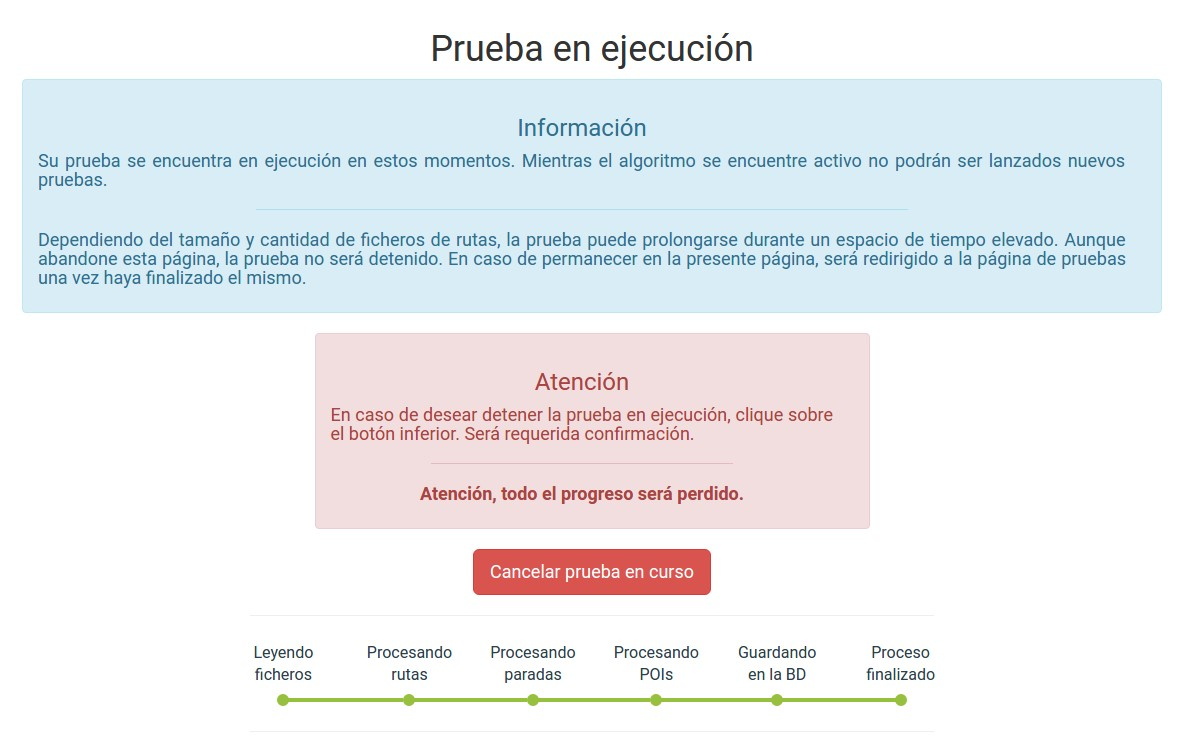
\includegraphics[width=0.6\textwidth]{../img/manualusuario/enejecucion.jpg}
  \caption{Algoritmo de análisis en ejecución.}
  \label{enejecucion}
\end{figure}

Una vez el proceso termina, se mostrará una nueva ventana indicando tal echo y se invitará al usuario a ver los resultados obtenidos.

\begin{figure}[h]
  \centering
    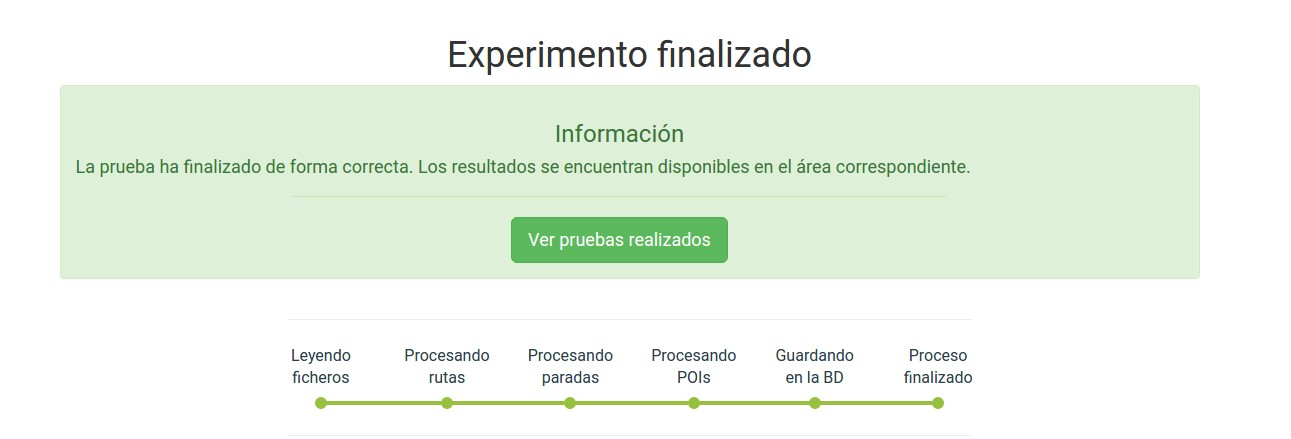
\includegraphics[width=0.6\textwidth]{../img/manualusuario/terminado.jpg}
  \caption{El algoritmo ha finalizado.}
  \label{terminado}
\end{figure}

\subsubsection{Visualización de resultados}
La pagina de visualización de resultados permite al usuario ver todas las rutas analizadas siendo dichas rutas mostradas de acuerdo al área seleccionada previamente. En la parte izquierda de la ventana se encontrarán las opciones de selección de área mientras que en la derecha se verán las rutas encontradas en el sistema. La Figura \ref{resultados} muestra una captura de esta página.

\begin{figure}[h]
  \centering
    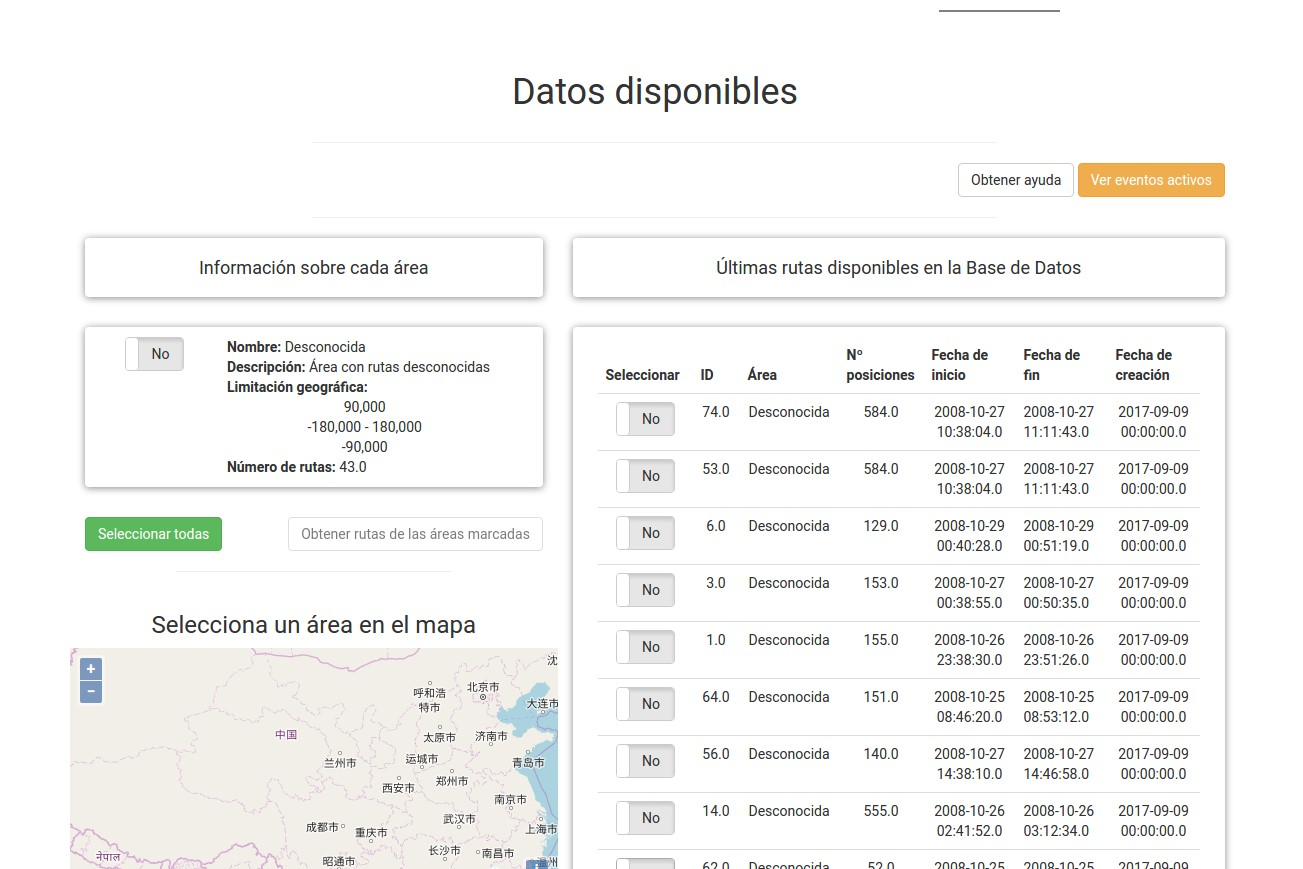
\includegraphics[width=0.6\textwidth]{../img/manualusuario/resultados.jpg}
  \caption{Página de resultados.}
  \label{resultados}
\end{figure}

Seleccionando una o varias áreas en la parte superior izquierda de la página habilitarán el botón inferior denominado \quotes{Obtener rutas de las áreas marcadas}. Una vez habilitado se podrá clicar y se buscarán las rutas pertenecientes a las áreas solicitadas. Si se prefiere, se puede hacer uso del mapa inferior o de las cajas de coordenadas de la parte final de la página. En la Figura \ref{mapacaja} se aprecia el mapa mencionado y las cajas de coordenadas.

\begin{figure}[h]
  \centering
    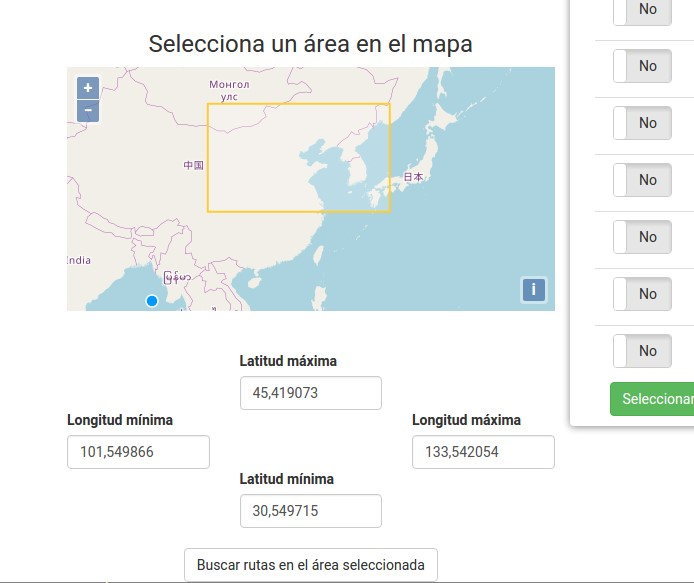
\includegraphics[width=0.6\textwidth]{../img/manualusuario/mapaycaja.jpg}
  \caption{Sección sobre el mapa.}
  \label{mapacaja}
\end{figure}

La selección sobre el mapa también mostrará las coordenadas elegidas sobre las cajas de coordenadas inferiores. El botón de búsqueda de rutas quedará activo y se podrá clicar para buscar las rutas en la Base de Datos.

La parte derecha de la página muestra las rutas que han sido filtradas. La tabla que se puede apreciar en la Figura \ref{vermas} cuenta con distintas columnas, estas son:

\begin{itemize}
	\item \textbf{Seleccionar:} permite seleccionar la ruta.
	\item \textbf{ID:} es el identificador de la ruta.
	\item \textbf{Área:} es el área asignada a la ruta.
	\item \textbf{Número de posiciones:} muestra el número de posiciones con las que cuenta la ruta.
	\item \textbf{Fecha de inicio:} fecha de inicio de la ruta (tomada de la primera posición de la misma).
	\item \textbf{Fecha de fin:} fecha de finalización de la ruta (tomada de la última posición de la ruta).
	\item \textbf{Fecha de creación:} es la fecha en la que se ha ejecutado el análisis.
\end{itemize}

Al seleccionar alguna de las rutas, el botón \quotes{Ver más detalles} queda activo permitiendo al usuario acceder a una última página. Esta página.

\begin{figure}[h]
  \centering
    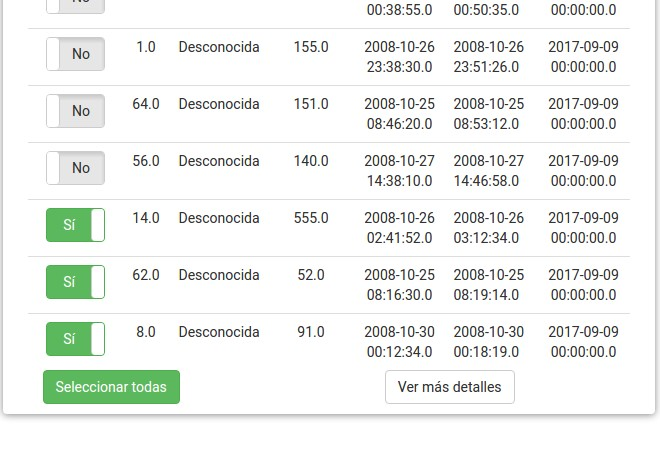
\includegraphics[width=0.6\textwidth]{../img/manualusuario/vermas.jpg}
  \caption{Botón que permite ver más detalles.}
  \label{vermas}
\end{figure}

Esta última página permitirá ver los detalles de las rutas seleccionadas y, además, se pintará sobre un mapa, dos marcadores mostrarán el inicio (verde) y fin (rojo) de cada ruta y una serie de marcadores adicionales mostrarán los PDIs cercanos, en caso de haber sido encontrados. El resultado podría ser similar al mostrado por la Figura \ref{rutaanalizada}.

\begin{figure}[h]
  \centering
    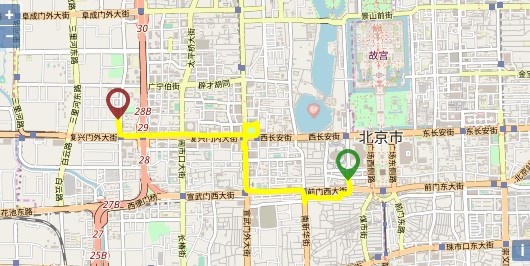
\includegraphics[width=0.6\textwidth]{../img/manualusuario/rutaanalizada.jpg}
  \caption{Una de las posibles rutas analizadas mostrada sobre un mapa.}
  \label{rutaanalizada}
\end{figure}


\subsubsection{Pruebas}
La página de pruebas permite visualizar todas las ejecuciones del algoritmo realizadas hasta el momento. Esta página (Figura \ref{ejecuciones}) permite ver en una tabla las opciones que han sido seleccionadas por cada ejecución. La siguiente lista detalla cada columna de esta tabla:

\begin{itemize}
	\item \textbf{Ficheros:} muestra el o los ficheros analizados. Para poder visualizar más de un fichero se ha de clicar sobre el botón \quotes{Ver todos}. Este botón indicará el número de ficheros analizados. Al clicar sobre el botón se lanzará un modal con el nombre de dichos ficheros.
	\item \textbf{Área:} muestra el nombre del área asignada a las rutas.
	\item \textbf{Distancia (rutas):} es la distancia máxima para dividir una ruta en dos partes.
	\item \textbf{¿Búsqueda de paradas?:} indica si el usuario ha realizado la búsquda de paradas.
	\item \textbf{Distancia:} es el valor que indica al algoritmo una distancia para considerar que dos puntos forman parte de una parada en ruta.
	\item \textbf{Variación de mediana:} valor que multiplica la mediana calculada
	\item \textbf{¿Búsqueda de POIs?:} indica si el usuario ha realizado la búsqueda de POIs.
	\item \textbf{Radio máximo:} valor que limita la búsqueda de Puntos De Interés en una parada.
	\item \textbf{Multiplicador de radio:} valor que multiplica al radio medido entre los puntos de una parada.
	\item \textbf{Almacenado en BD:} indica si los resultados han sido almacenado en la Base de Datos.
	\item \textbf{Fecha de la prueba:} fecha en la que se ha llevado a cabo la prueba.
	\item \textbf{Repetir / Eliminar:} botones que permiten repetir o eliminar la prueba.
\end{itemize}

\begin{figure}[h]
  \centering
    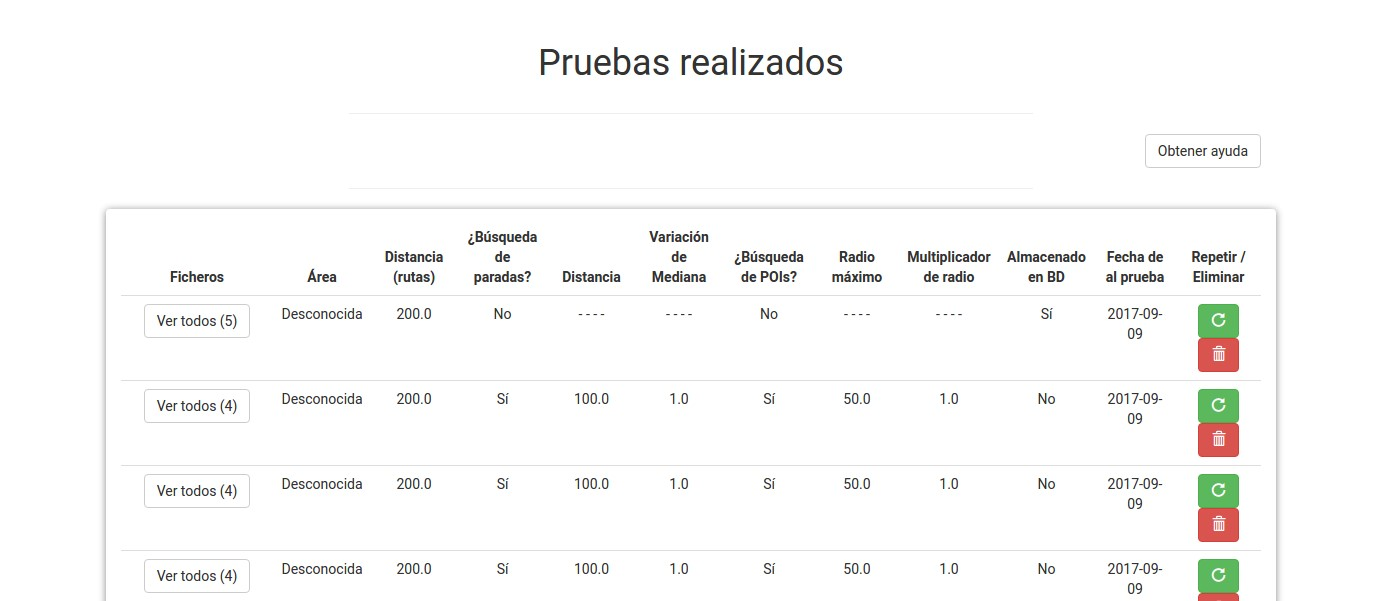
\includegraphics[width=0.6\textwidth]{../img/manualusuario/ejecuciones.jpg}
  \caption{Tabla de pruebas ejecutadas.}
  \label{ejecuciones}
\end{figure}

El botón inferior con texto \quotes{Eliminar todas las pruebas realizadas} permite eliminar todas las filas de la tabla de una sola vez. La Figura \ref{borratodaspruebas} muestra este botón. Se lanzará un modal como el apreciable en la Figura \ref{borradopruebasmodal} para asegurar el borrado de estas pruebas.

\begin{figure}[h]
  \centering
    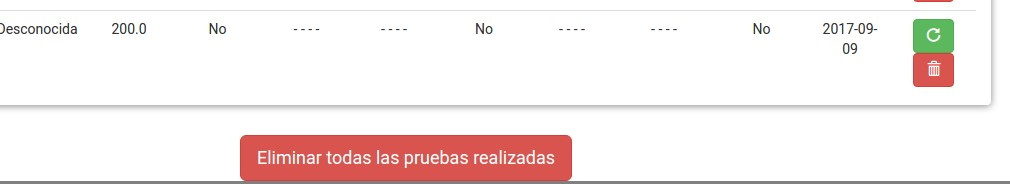
\includegraphics[width=0.6\textwidth]{../img/manualusuario/borratodaspruebas.jpg}
  \caption{Botón de borrado total de pruebas.}
  \label{borratodaspruebas}
\end{figure}

\begin{figure}[h]
  \centering
    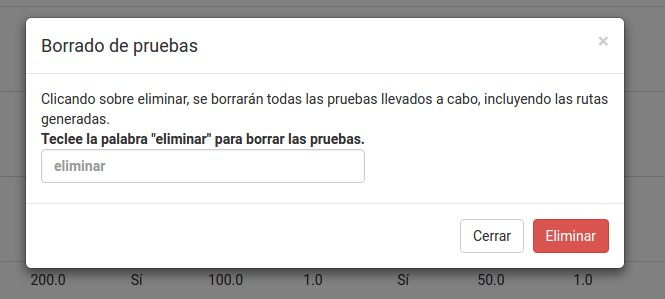
\includegraphics[width=0.6\textwidth]{../img/manualusuario/borradopruebasmodal.jpg}
  \caption{Modal de borrado de pruebas.}
  \label{borradopruebasmodal}
\end{figure}

\subsubsection{Gestión}
Como muestra la Figura \ref{manage}, la página de sección queda dividida en tres grandes grupos: Gestión de áreas, Gestión de Puntos de Interés y Borrado de datos

\begin{figure}[h]
  \centering
    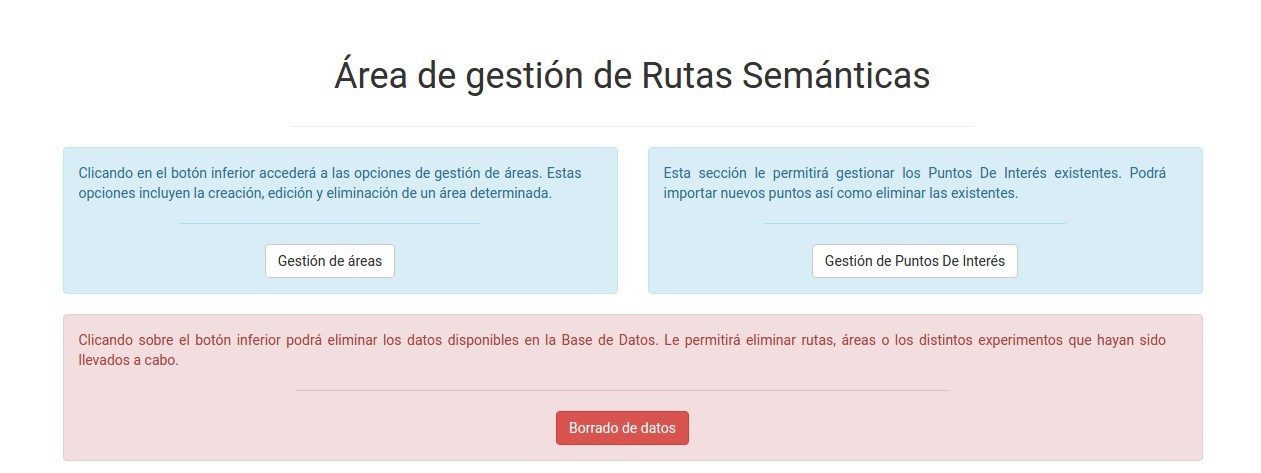
\includegraphics[width=0.6\textwidth]{../img/manualusuario/manage.jpg}
  \caption{Gestión de la plataforma web.}
  \label{manage}
\end{figure}

Accediendo a cada sección se podrá gestionar cada uno de los aspectos mencionados.

\paragraph{Gestión de áreas:} la sección de gestión de áreas permite visualizar las áreas existentes, modificar cada una de las creadas con anterioridad, eliminar alguna de las áreas no deseadas o crear un nuevo área. En la Figura \ref{areamanage1} se puede ver esta página.

\begin{figure}[h]
  \centering
    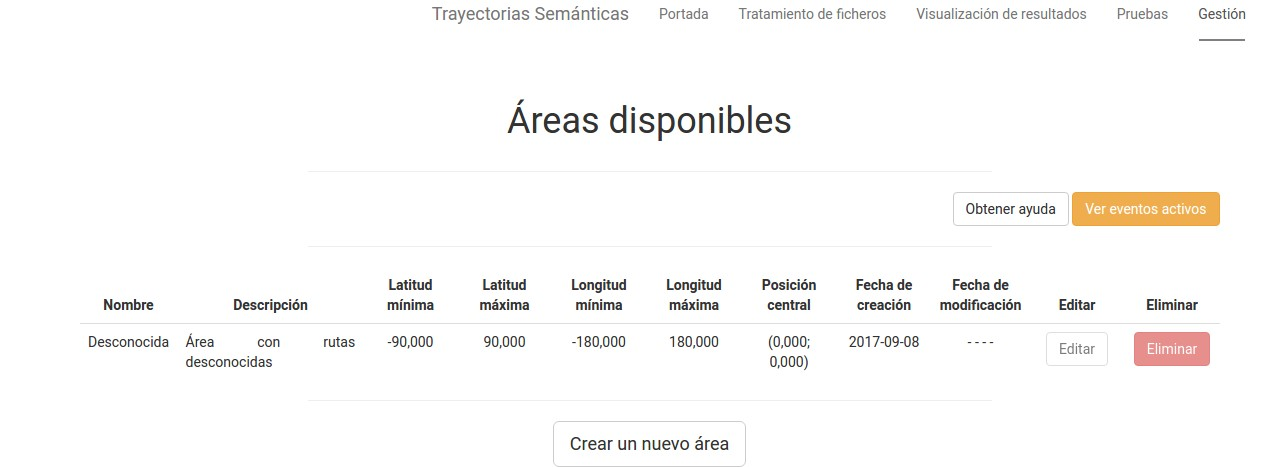
\includegraphics[width=0.6\textwidth]{../img/manualusuario/areamanage1.jpg}
  \caption{Gestión de áreas.}
  \label{areamanage1}
\end{figure}
 
La tabla muestra el nombre del área, su descripción, la localización geográfica mediante los límites que muestran sus coordenadas geográficas, la fecha de creación del área y la fecha de modificación de la misma en caso de haber sufrido alguna modificación. También se observan dos botones: edición y borrado. Mediante el botón de edición se permite al usuario editar todos los valores relacionados con el área en cuestión. El botón de borrado permitirá eliminar el área seleccionada.

Clicando sobre el botón de edición se mostrará la ventana emergente que referencia la Figura \ref{areaedit}. 

\begin{figure}[h]
  \centering
    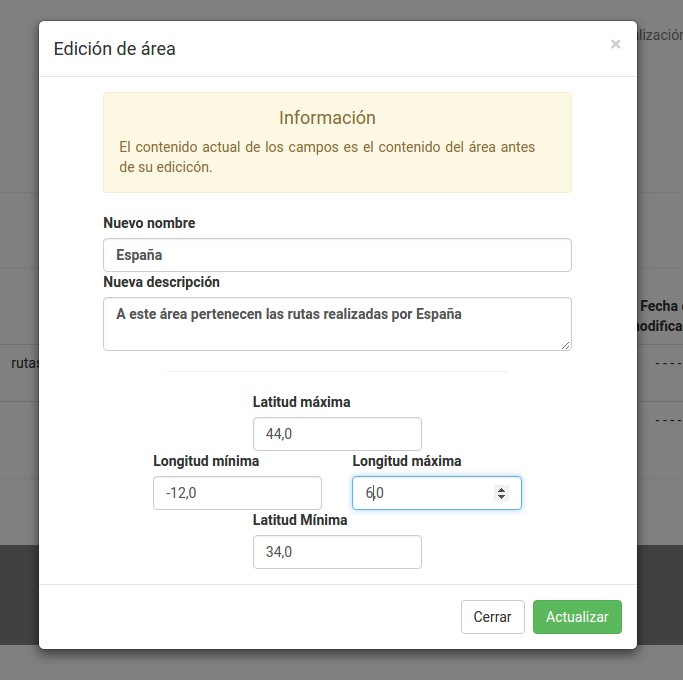
\includegraphics[width=0.6\textwidth]{../img/manualusuario/areaedit.jpg}
  \caption{Edición de área existente.}
  \label{areaedit}
\end{figure}

Si se desea crear una nueva área, simplemente se ha de clicar sobre el botón correspondiente (\quotes{Crear un nuevo área}) y se mostrará el mismo modal que para la edición salvo que sus entradas de texto y/o número estarán vacías. Al crear el área aparecerá de forma inmediata en el listado mostrado por la tabla de áreas.

Para eliminar un área bastará con clicar sobre el botón de borrado correspondiente a cada área y aceptar la solicitud que indica el modal.

\paragraph{Gestión de Puntos de Interés:} Un aspecto fundamental en este trabajo es el manejo de Puntos De Interés por parte del sistema. Para que el usuario pueda cargar nuevos PDIs en la Base de Datos se cuenta con el sencillo formulario ubicado en esta página. Como se puede apreciar en la Figura \ref{pdimanage}, simplemente se ha de seleccionar un fichero de tipo xml que cuente con los PDIs a subir e indicar un nombre de región en la que los distintos PDIs están englobados. Por ejemplo, si se desean cargar PDIs de España, se seleccionará el fichero xml y se indicará como región España. De esta forma, si el usuario desea eliminar alguna de las regiones, puede diferenciarla de forma sencilla y clara.

\begin{figure}[h]
  \centering
    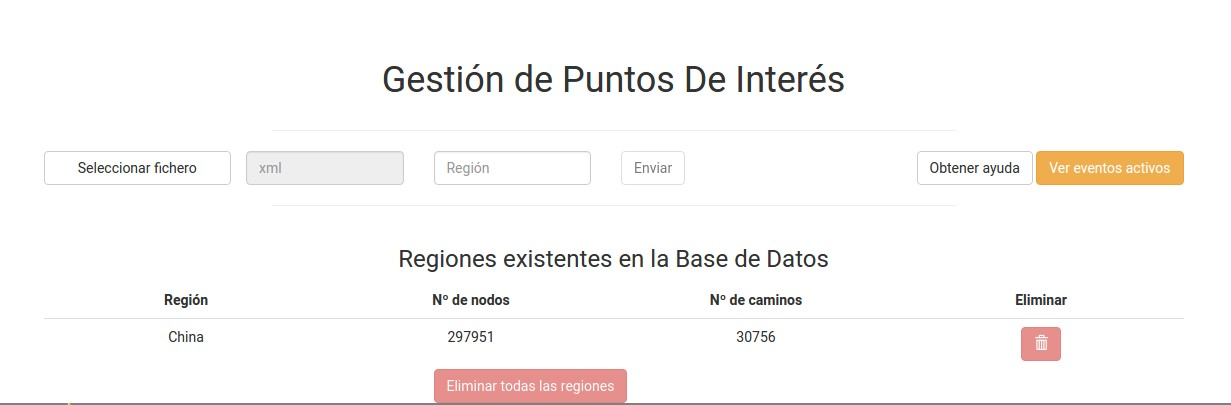
\includegraphics[width=0.6\textwidth]{../img/manualusuario/pdimanage.jpg}
  \caption{Gestión de PDIs.}
  \label{pdimanage}
\end{figure}

Clicando sobre el botón \quotes{Enviar} se procederá a la carga de los datos del fichero seleccionado. Se puede ver cómo evoluciona el proceso en la ventana que muestra el navegador mientras el proceso se encuentra activo. Es apreciable en la Figura \ref{pdimanage2}.

\begin{figure}[h]
  \centering
    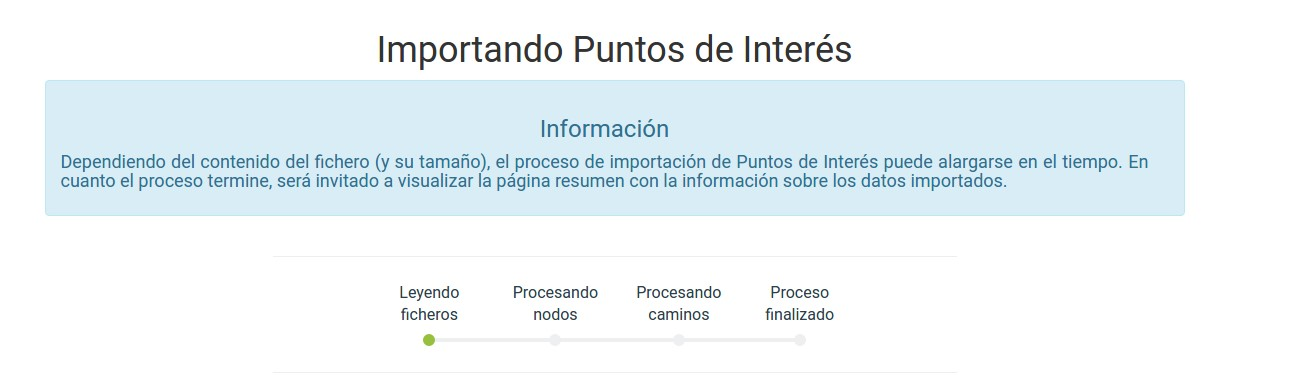
\includegraphics[width=0.6\textwidth]{../img/manualusuario/pdimanage2.jpg}
  \caption{Subida de PDIs.}
  \label{pdimanage2}
\end{figure}

Una vez haya finalizado el proceso, la nueva región aparecerá en la tabla de regiones de esta página y se mostrarán el total de Puntos De Interés y caminos (Ways) con los que cuenta. Para eliminar una o varias regiones se debe clicar en el botón de borrado correspondiente a cada una o en el botón de borrado total situado en la parte inferior de la página.

\paragraph{Borrado de datos:} se proporciona una página especialmente diseñada que permite eliminar completamente todos los datos del sistema. Cuenta con dos secciones, la primera permite eliminar únicamente los Puntos De Interés almacenados (obviamente, elimina todas las regiones creadas por el usuario). La segunda sección permite vaciar las tablas de rutas, pruebas, etc y, además, permite eliminar los ficheros que han sido subidos al servidor. La Figura \ref{deleteall} permite ver una captura de esta página de la plataforma web.

\begin{figure}[h]
  \centering
    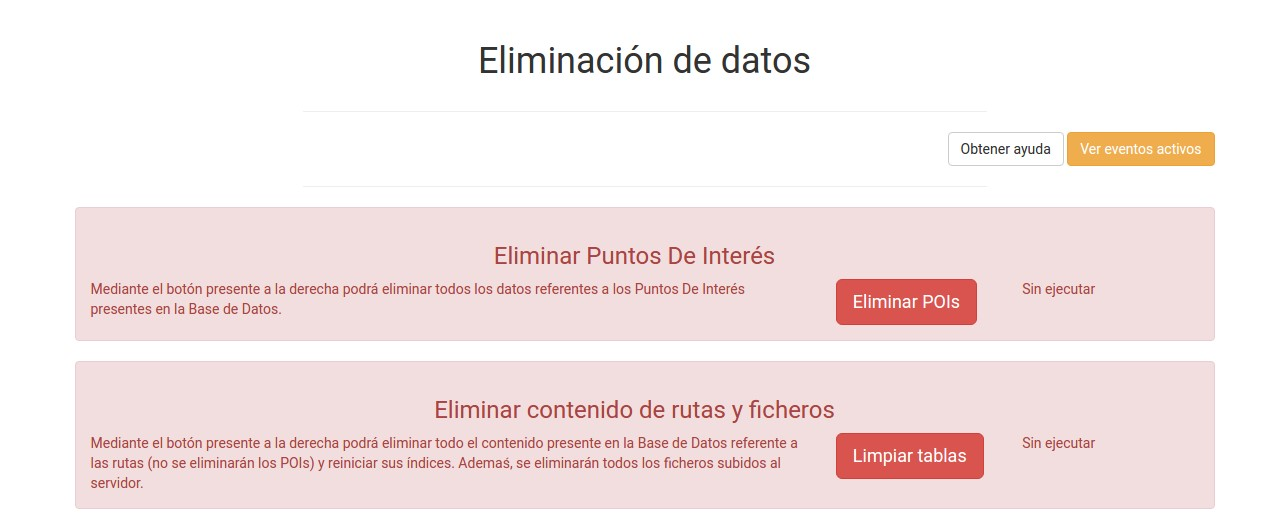
\includegraphics[width=0.6\textwidth]{../img/manualusuario/deleteall.jpg}
  \caption{Borrado de datos.}
  \label{deleteall}
\end{figure}

Es importante tener en cuenta que si una prueba o una carga de Puntos De Interés está activa, los hilos de ejecución correspondientes serán parados y se procederá al borrado de los datos.

Se mostrará un modal advirtiendo del borrado que se va a realizar evitando el borrado accidental de datos correctos.


\section{Obtención y manipulación de datos}
La plataforma web anteriormente descrita necesita diferentes datos para resultar útil. El primer conjunto de datos necesarios para poder llevar a cabo un análisis de rutas es el correspondiente a los Puntos De Interés que se deseen localizar en las paradas de las rutas. Este conjunto de datos puede obtenerse a partir de ficheros de tipo \textbf{osm}. En las siguientes secciones se explica cómo obtener estos datos.

El segundo conjunto de datos necesario es el de las rutas propiamente dichas. Para realizar las pruebas se han buscado en distintos lugares de internet el mejor conjunto de datos posibles. En la parte final de este aenxo se mencionan los conjuntos de datos analizados y por qué se ha escogido uno en concreto.

A continuación se muestra cómo obtener un mapa completo de China en formato comprimido (\textbf{pbf}), después se indicará cómo convertir este formato a osm y, por último, cómo obtener su conjunto de Puntos De Interés.

\subsection{Descarga de mapas}
Accediendo a la web de descargas de Geofabrik (enlace: \url{http://download.geofabrik.de/}) será posible elegir el país o continente cuyo mapa se desea descargar. La página principal de descargas permite obtener un continente completo (se aprecia en la Figura \ref{asaia1}). En esta ocasión se desea obtener solamente el mapa correspondiente a China. Por tanto, se clica sobre la fila correspondiente a Asia y en la segunda página se clica sobre China. El proceso es el descrito en las figuras \ref{asia2} y \ref{asia3}.

\begin{figure}[h]
  \centering
    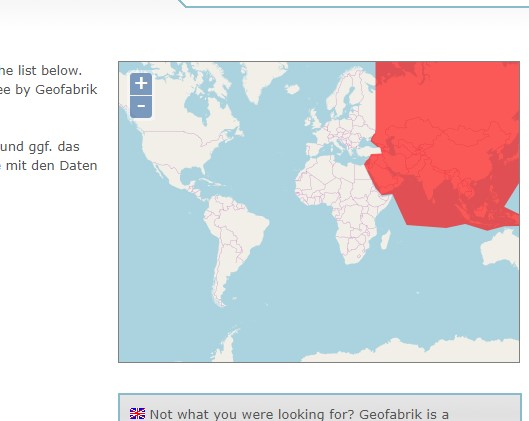
\includegraphics[width=0.6\textwidth]{../img/manualusuario/asia1.jpg}
  \caption{Continente asiático.}
  \label{asia1}
\end{figure}

\begin{figure}[h]
  \centering
    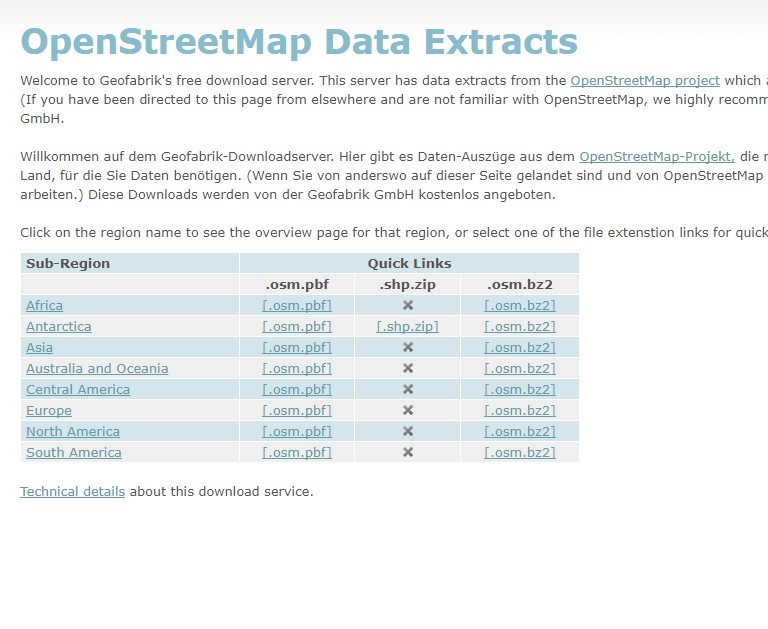
\includegraphics[width=0.6\textwidth]{../img/manualusuario/asia2.jpg}
  \caption{Tabla mostrando todos los continentes.}
  \label{asia2}
\end{figure}

\begin{figure}[h]
  \centering
    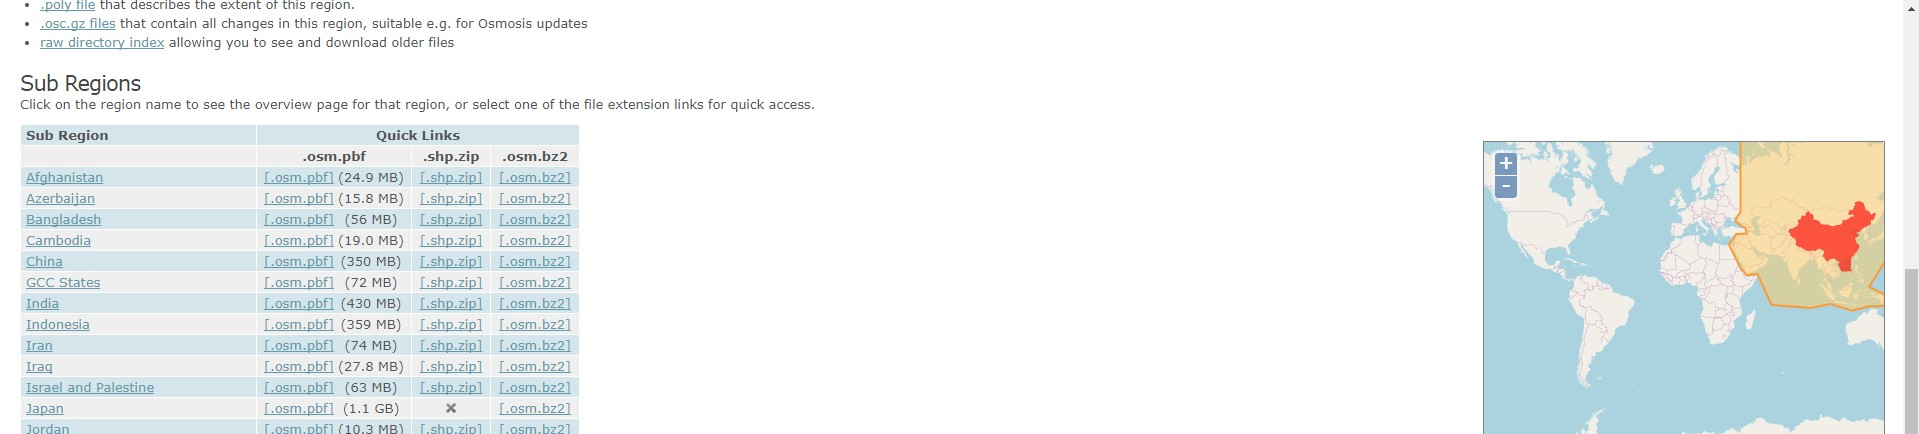
\includegraphics[width=0.6\textwidth]{../img/manualusuario/asia3.jpg}
  \caption{Tabla con los países asiáticos.}
  \label{asia3}
\end{figure}


Una vez descargado el mapa de China en formato pbf (ocupa unas 350 MiB), se puede subdividir mediante la herramienta Osmosis. De esta forma se podrán extraer ciudades del interior del país, regiones o provincias, etc.

Antes de continuar y, como será necesario en los siguientes pasos, se usará la herramienta \textit{osmconvert} para convertir el mapa descargado a un fichero de tipo osm.

\subsubsection{Osmconvert}
El ejemplo de uso de la herramienta \textit{osmconvert} partirá de un fichero llamado \textbf{china-latest.osm.pbf} que será convertido a china-latest.osm. El comando a usar, si el usuario se encuentra situado en la carpeta donde se encuentra el fichero pbf es el siguiente:

\begin{lstlisting}[language=bash]
	osmconvert china-latest.osm.pbf --out-osm -o=china-latest.osm
\end{lstlisting}

Este comando necesita que se le indique el nombre del fichero de salida y su formato. Para convertir mapas de otros países o continentes es suficiente con cambiar los valores del mapa de entrada y el nombre del fichero de salida.

El proceso puede tardar unos segundos debido a que es posible que se genere un fichero de dimensiones considerables. En este caso, se pasa de un archivo de unas 350 MiB a uno de más de 8 GiB de extensión.

En este momento se está en disposición de hacer uso de dos herramientas, la primera, que es \quotes{Osmosis}, permitirá extraer una zona del mapa de China. La segunda, \quotes{Osmfilter}, permite obtener los Puntos De Interés a partir del mapa en formato osm. Como ejemplo, se extraerá la ciudad de Pekín a partir del fichero osm obtenido en este paso.

\subsection{Osmosis}
Osmosis permite extraer una zona concreta de un mapa con extensión osm o pbf. A continuación y, a como ejemplo, se muestran los pasos necesarios para obtener la zona correspondiente a una  ciudad concreta, en este caso Pekín, partiendo de un mapa completo de China.

\subsubsection{Extracción de una ciudad}
Para extraer una ciudad del plano que se acaba de descargar se ha de abrir la consola del sistema y hacer uso de la herramienta Osmosis. Se necesitarán los siguientes argumentos (entre paréntesis las coordenadas que serán usadas en el caso de Pekín):
\begin{itemize}
	\item Nombre del fichero de entrada: se seleccionará el fichero de extensión osm sobre el que se obtendrá el recorte del mapa.
	\item Coordenada GPS que indique la parte \textbf{superior} del segmento de mapa que se va a recortar (41.3).
	\item Coordenada GPS que indique la parte \textbf{izquierda} del segmento de mapa que se va a recortar (115.0).
	\item Coordenada GPS que indique la parte \textbf{inferior} del segmento de mapa que se va a recortar (39.4).
	\item Coordenada GPS que indique la parte \textbf{derecha} del segmento de mapa que se va a recortar (117.35).
	\item Nombre del fichero de salida: se dará nombre al fichero de salida con extensión osm.
\end{itemize}

El comando a teclear incluirá los siguientes parámetros:
\begin{itemize}
	\item rb: permite leer el contenido del fichero pbf descargado.
	\item bb: permite extraer los datos indicados en la caja definida por las coordenadas geográficas indicadas a continuación.
	\item top: coordenada geográfica superior.
	\item right: coordenada geográfica derecha.
	\item bottom: coordenada geográfica inferior.
	\item left: coordenada geográfica izquierda.
	\item wx: permite escribir los datos en un fichero osm.
\end{itemize}

Una vez descritos los parámetros y valores necesarios, se ejecuta el comando de la siguiente forma:

\begin{lstlisting}[language=bash]
	osmosis --read-xml china-latest.osm --bb top=41.3 left=115.0 bottom=39.4 right=117.35 --wx pekin.osm
\end{lstlisting}

El proceso puede tardar unos instantes debido a que el tamaño del fichero inicial es grande. Una vez lanzado el comando, se verá la siguiente salida por consola:

\begin{figure}[h]
  \centering
    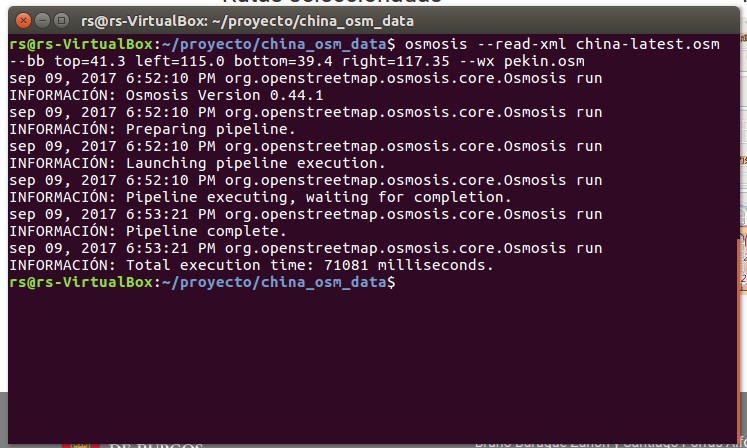
\includegraphics[width=0.6\textwidth]{../img/osmextract/osmosis.jpg}
  \caption{Impresión en consola del resultado del comando.}
  \label{puntosGeograficos}
\end{figure}

\subsection{Osmconvert}
Es el momento de obtener los datos correspondientes a los Puntos De Interés de la ciudad de Pekín. El comando para esta herramienta es sencillo, en la siguiente lista se muestran los parámetros necesarios:

\begin{itemize}
	\item \textbf{Fichero de entrada osm:} es el fichero de entrada que se proporcionará a la herramienta, en este ejemplo, Pekin.osm.
	\item \textbf{Opciones \quotes{keep}:} \textit{keep} indica los nodos a mantener. En este caso se seleccionan los nodos, caminos y relaciones que incluyen una etiqueta de tipo amenity. Esta etiqueta es una descripción general del nodo (Catedral, Universidad, etc).
	\item \textbf{Fichero de salida (xml):} se ha de indicar como salida un nombre de fichero en formato xml.
\end{itemize}

El comando quedaría de la siguiente forma:

\begin{lstlisting}[language=bash]
	osmfilter pekin.osm --keep="amenity=" --keep-ways="amenity=" --keep-relations="amenity=" > pekin-pois.xml
\end{lstlisting}

Siendo l resultado por consola es el mostrado en la Figura \ref{filter}.
\begin{figure}[h]
  \centering
    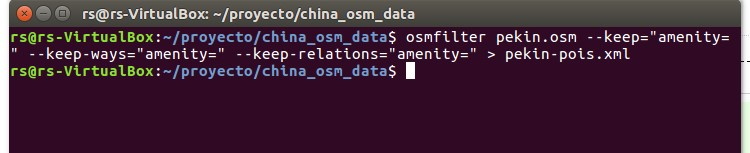
\includegraphics[width=0.6\textwidth]{../img/osmextract/filter.jpg}
  \caption{Impresión en consola del resultado del comando osmfilter.}
  \label{filter}
\end{figure}

Si se desea subir este fichero de Puntos De Interés a la plataforma web, simplemente se ha de abrir la página de Gestión de Puntos De Interés y proceder a su subida, las figuras \ref{subida1}, \ref{subida2}, \ref{subida3} muestran el proceso que puede extenderse en el tiempo dependiendo del tamaño del fichero xml procesado.

\begin{figure}[h]
  \centering
    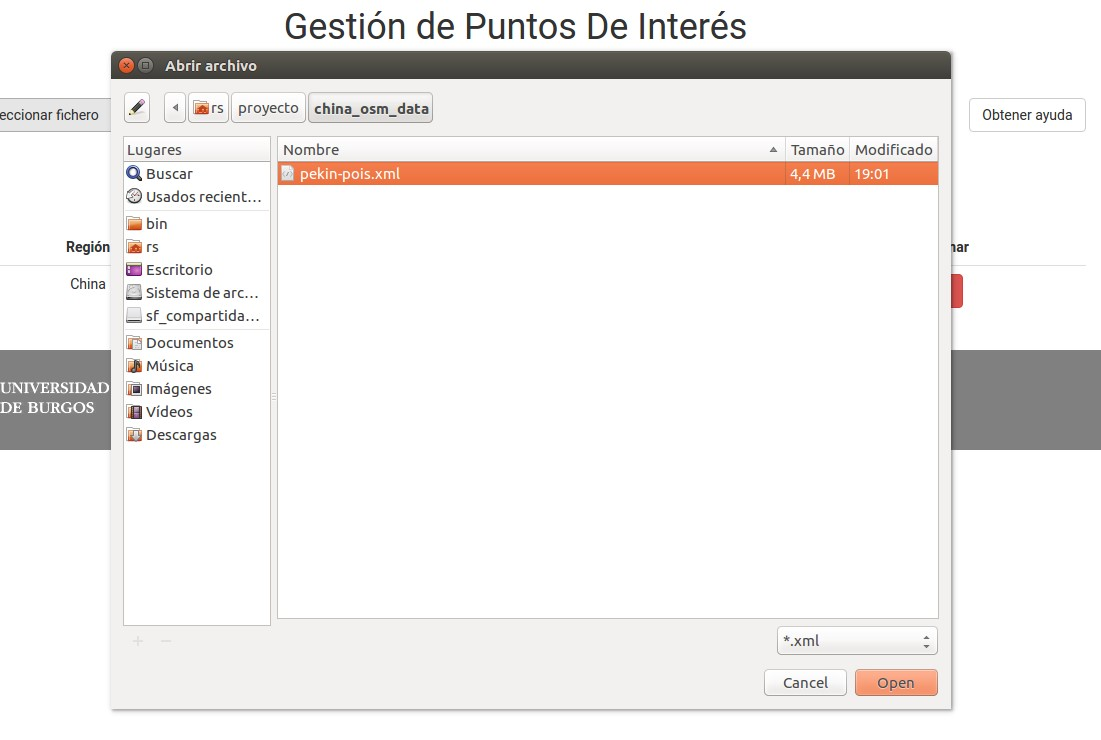
\includegraphics[width=0.6\textwidth]{../img/osmextract/subida1.jpg}
  \caption{Selección del fichero.}
  \label{subida1}
\end{figure}
\begin{figure}[h]
  \centering
    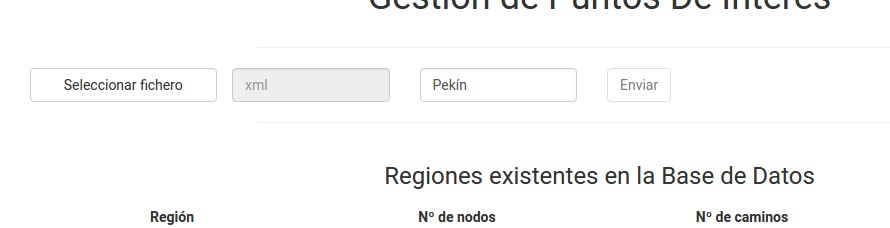
\includegraphics[width=0.6\textwidth]{../img/osmextract/subida2.jpg}
  \caption{Región a la que pertenece.}
  \label{subida2}
\end{figure}
\begin{figure}[h]
  \centering
    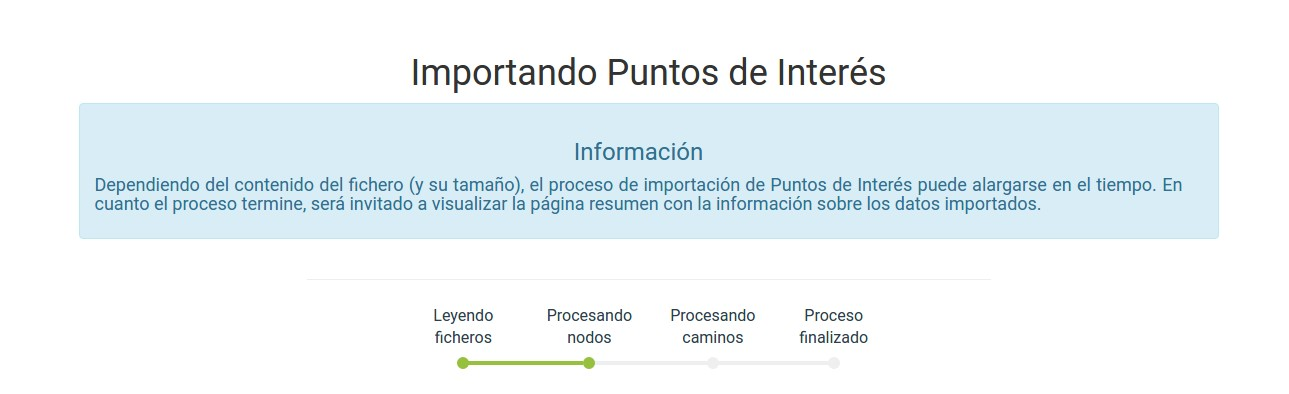
\includegraphics[width=0.6\textwidth]{../img/osmextract/subida3.jpg}
  \caption{Ejecución del procesado.}
  \label{subida3}
\end{figure}
Una vez finalice el proceso, la nueva región quedará visible en la tabla de regiones. Para que no existan PDIs duplicados se omitirá el guardado de nodos existentes.



\section{QGIS}
Como se ha comentado a lo largo de esta documentación, QGIS es un excelente programa en el que visualizar mapas, rutas, etc. Por tanto, se hará un breve resumen de las opciones principales con las que el usuario cuenta al hacer uso de dicho programa.

\subsection{QGIS}
QGIS es una herramienta de información geográfica libre y de código abierto que permite conexiones con PostgreSQL y visualización de los datos obtenidos sobre un mapa físico. 

También permite la obtención de información geográfica desde Open Street Maps. De esta forma se pueden superponer rutas/trazas obtenidas desde las tablas de la Base de Datos con los mapas de Open Street Maps.

Para configurar una conexión contra la Base de Datos instalada y configurada anteriormente se ha de clicar en el icono de PostgreSQL ubicado en la columna central izquierda. Pedirá al usuario una serie de valores como:

\begin{itemize}
\item \textbf{nombre:} valor que se dará al nombre de la conexión (localhost).
\item \textbf{servidor:} servidor contra el que se realizará la conexión. En este caso será el servidor local (localhost).
\item \textbf{Base de datos:} la Base de Datos de la que serán obtenidos los datos (rutassemanticas).
\item \textbf{Autenticación:} nombre de usuario y contraseña  del usuario de PostgresQL usado para obtener la información (rs, rs).
\end{itemize}

La Figura \ref{conexionqgis} muestra la ventana emergente que permite realizar la conexión con los valores ya introducidos.

\begin{figure}[h]
  \centering
    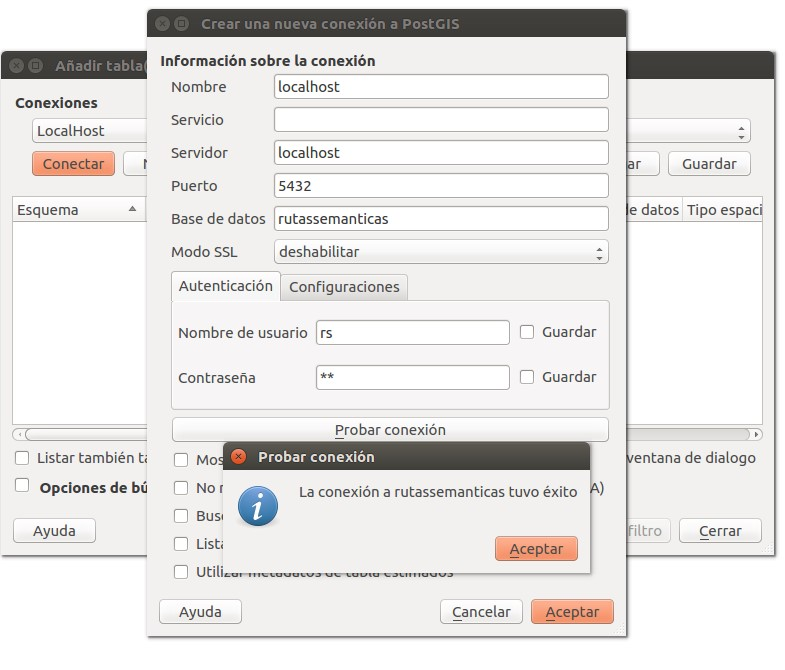
\includegraphics[width=0.6\textwidth]{../img/qgis/conexionqgis.jpg}
  \caption{Conexión contra PostgreSQL en QGIS.}
  \label{conexionqgis}
\end{figure}

Una vez se consigue una conexión, aparecerán las tablas que en la Base de Datos cuentan con columnas representables por QGIS, esto es, la tabla que se desee usar ha de contar con una columna de tipo \quotes{the\_geom}. Este tipo de dato es propio de PostGIS y permite situar coordenadas geográficas de una forma sencilla y rápida para el sistema.

Otro de los aspectos importantes a tener en cuenta es la facilidad que brinda al usuario para descargar contenido en formato osm indicando una zona determinada mediante coordenadas geográficas. Esta característica ofrece el mismo resultado que el recorte del mapa de China realizado con Osmosis. A continuación, se muestra un ejemplo con los mismos datos.

\subsubsection{Descarga de contenido OSM con QGIS}
Para comenzar, se ha de acceder a la sección ``Vectorial'', después, situar el cursor sobre ``OpenStreetMaps'' y clicar sobre ``Descargar datos'' (Figura \ref{vectorial}).

\begin{figure}[h]
  \centering
    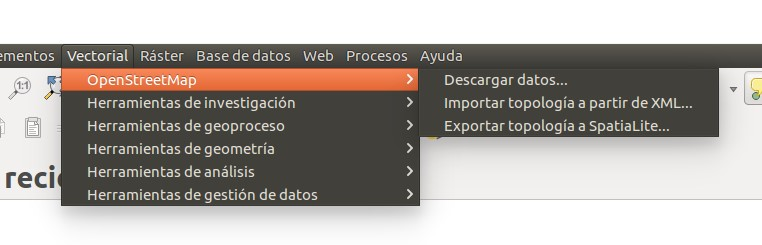
\includegraphics[width=0.8\textwidth]{../img/qgis/descarga.jpg}
  \caption{Descarga de datos desde QGIS}
  \label{vectorial}
\end{figure}

A continuación se indicarán las coordenadas sobre las que se desea obtener los datos. En la Figura \ref{datos} se indican sus valores, son los mismos que los usados en Osmosis. Además, se ha de seleccionar un fichero destino. En este caso, se aprecia que es el mismo que el descargado mediante Osmosis.

\begin{figure}[h]
  \centering
    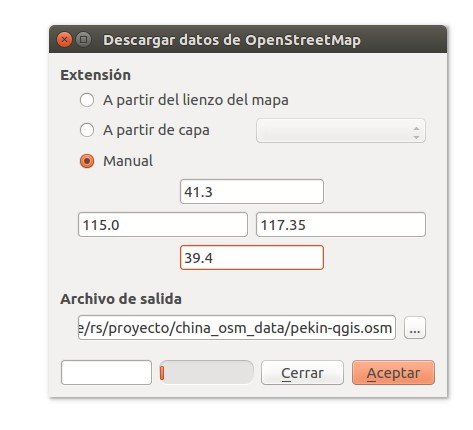
\includegraphics[width=0.8\textwidth]{../img/qgis/pekin-qgis.jpg}
  \caption{Valores introducidos para la búsqueda de datos en QGIS}
  \label{datos}
\end{figure}

\begin{figure}[h]
  \centering
    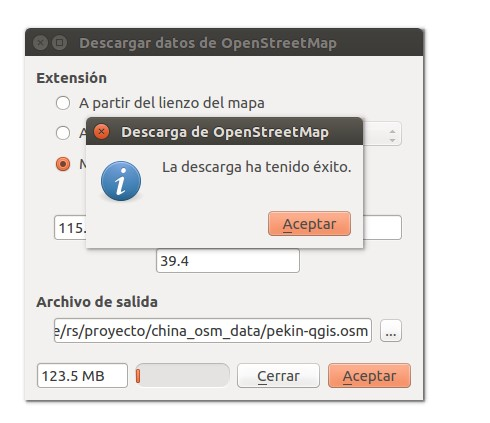
\includegraphics[width=0.8\textwidth]{../img/qgis/exito.jpg}
  \caption{Éxito en la descarga de los datos.}
  \label{exito}
\end{figure}
Por último, se mostrará un mensaje de éxito si todo ha salido correctamente (Figura \ref{exito}).

Ahora se cuenta con el mismo fichero de extensión OSM y será posible extraer los datos referentes a Puntos De Interés de la forma ya mencionada.

Para obtener más información sobre QGIS se puede acceder al siguiente enlace: \url{http://www.qgis.org/es/docs/index.html}.



\section{Datos de prueba}
Esta sección pretende ilustrar cómo se han obtenido los datos con los que se han realizado las pruebas. De esta forma un futuro usuario podrá navegar por las páginas aquí mencionadas y tener una base para obtener nuevos datos de prueba para esta plataforma o para cualquier otra.


\subsection{Origen de datos}
El problema inicial al que hacer frente ha sido la falta de datos propios como punto de partida, por tanto, se ha tenido que realizar una búsqueda en distintos sitios de Internet para conseguir un conjunto de datos lo más fiables posible y con la estructura adecuada. Se han establecido una serie de condiciones indispensables que el \textit{dataset} ha de cumplir:
\begin{itemize}
\item \textbf{Coordenadas geográficas:} cada coordenada ha de contar con una latitud y longitud separadas en dos campos.
\item \textbf{Marca de tiempo:} cada una de las coordenadas geográficas incluidas ha de contar con una marca de tiempo que permita localizar la coordenada en un espacio temporal concreto (un día, una semana, etc.).
\item \textbf{Altitud:} para que la coordenada geográfica sea más precisa, debe contar con su altitud.
\item \textbf{Diferenciación de rutas:} de igual manera que una coordenada geográfica se ha de poder diferencia de la siguiente, cada ruta incluida en el \textit{dataset} ha de poder ser diferenciada del resto. Es importante que cada una de las rutas se diferencien mediante un identificador único o se encuentren en ficheros separados.
\end{itemize}

Algunos de los sitios donde se pueden buscar este tipo de \textit{dataset} incluyen páginas como el repositorio de Machine Learning de la Universidad Irvine de California (\url{http://archive.ics.uci.edu/ml/}). Donde se pueden encontrar los últimos \textit{dataset} subidos o un buscador para poder encontrar el \textit{dataset} buscado. En esta página se han encontrado y valorado dos conjuntos de datos.

\subsubsection{Taxi Service Trajectory}
El primer \textit{dataset} encontrado ha sido el correspondiente a distintos trayectos en taxi sobre la ciudad de Oporto (Portugal). Este conjunto de datos se compone de un amplio fichero csv con información como el tipo de llamada realizada a la compañía de taxis, el taxi que ha respondido a la misma, la fecha y hora a la que se produjo la llamada y el conjunto de coordenadas geográficas tomadas durante el trayecto.

Aunque el conjunto de los datos parece interesante en un primer momento, no se cuenta con un indicador temporal por cada coordenada y los hace inviables para su posterior uso, siendo este el motivo por el que se ha descartado el uso de este conjunto de datos.

Este dataset puede ser descargado desde el siguiente enlace: \url{https://archive.ics.uci.edu/ml/datasets/Taxi+Service+Trajectory+-+Prediction+Challenge,+ECML+PKDD+2015}.

\subsubsection{GPS Trajectories Data Set}
El segundo de los conjuntos de datos analizados ha sido el correspondiente a las rutas realizadas por un conjunto de usuarios en la ciudad de Aracaju (Brasil) en taxi o autobús. Estos datos se encuentran divididos en dos ficheros csv. El primero de los ficheros cuenta con un identificador único de usuario, de esta forma se puede conocer qué usuario ha tomado cada ruta, un indicador de velocidad de la ruta (inicialmente no necesario), un campo de tiempo, uno de distancia recorrida, algunos de calificación de la ruta (rating) y por último, uno indicando la línea de autobús en la que se ha realizado el trayecto.

El segundo de los ficheros incluye cada una de las coordenadas geográficas correspondientes a cada ruta y su asociación al usuario que la ha tomado.

Aunque inicialmente fue uno de los \textbf{dataset} tenidos en cuenta, se ha desechado por no contener un número elevado de rutas que permitiese una mayor aleatoriedad en los datos.

Este conjunto de datos puede ser descargado desde el siguiente enlace: \url{https://archive.ics.uci.edu/ml/datasets/GPS+Trajectories}.

\subsubsection{Geolife}
El \textit{dataset} seleccionado ha sido el denominado Geolife GPS Trajectories. Este dataset pertenece al repositorio que mantiene Microsoft. Este conjunto de datos viene acompañado por un documento en el que se indica cómo se han obtenido los datos, cuál es su estructura, etc. Se menciona que los datos han sido recolectados por unos 180 usuarios, en su mayoría en la ciudad de Pekín (China) pero también existen datos de viajes a otras ciudades o, incluso, a otros países.

En el \textit{dataset} se incluye una carpeta por cada usuario y en cada carpeta se puede encontrar un fichero que toma su nombre de la marca de tiempo de la primera coordenada de cada ruta. Por tanto, puede que un usuario cuente con un único fichero, indicando así que solo ha realizado una ruta, o que cuente con múltiples ficheros en los que se almacenan distintas rutas.

Cada fichero contiene una línea por cada coordenada geográfica obtenida. Esta línea contiene distinta información: un par latitud longitud, que permite situar la coordenada geográfica sobre un plano, su altitud y su marca temporal (entre otras). Esta estructura hace que la diferenciación de las rutas sea sencilla ya que se encuentran separadas por usuarios y marca temporal en la que ha sido tomada. Debido a esto, este conjunto de datos es el que ha sido finalmente elegido y volcado a la Base de Datos.

Finalmente, comentar que otras universidades como la de St Andrews (\url{https://uk.crawdad.org/}) también prestan sus \textit{dataset} aunque, en esta ocasión, no se ha revisado su repositorio en profundidad.



\bibliographystyle{plain}
\bibliography{bibliografiaAnexos}

\end{document}